\documentclass{ctexart}

\usepackage{van-de-la-sehen}
\usepackage{van-le-trompe-loeil}

\begin{document}

\section{Lagrange方程的应用} % (fold)
\label{sec:lagrange方程的应用}

\subsection{有心力} % (fold)
\label{sub:有心力}

\subsubsection{两体问题} % (fold)
\label{ssub:两体问题}

\begin{figure}[ht]
    \centering
    \incfig{8cm}{InCOMF}
\end{figure}
在只有内部相互作用的情形下, $V = V\pare{\+vr_1 - \+vr_2}$. 设定相对位移$\+vr = \+vr_1 - \+vr_2$, 质心
\[ \+vr_c = \frac{m_1\+vr_1 + m_2\+vr_2}{m_1+m_2}. \]
在广义坐标变换$\pare{\+vr_1,\+vr_2}\mapsto \pare{\+vr_c,\+vr}$下,
\begin{align*}
    L &= \half m_1\pare{\dot{\+vr}_c + \frac{m_2}{m_1+m_2}\dot{\+vr}}^2 + \half m_2 \pare{\dot{\+vr}_c - \frac{m_1}{m_1+m_2}\dot{\+vr}}^2 \\
    &= \half\pare{m_1+m_2}\dot{\+vr}_c^2 + \half m\dot{\+vr}^2 - V\pare{\+vr}.
\end{align*}
其中$\displaystyle m = \frac{m_1m_2}{m_1+m_2}$是两者的约化质量. 由于质心惯性运动, 可以取$\+vr_c \equiv 0$, 从而
\[ L' = \half m\dot{\+vr}^2 - V\pare{\+vr}. \]
\begin{remark}
    $\+vp_c = \pare{m_1+m_2}\dot{\+vr_c} \neq m\dot{\+vr}$.
\end{remark}
若$V$是旋转对称的, 即$V = V\pare{\abs{\+vr}}$, 则系统谓有心力系统.

% subsubsection 两体问题 (end)

\subsubsection{有心力系统} % (fold)
\label{ssub:有心力系统}

对于有心力系统, $\displaystyle L = \half m\dot{\+vr}^2 - V\pare{r}$. 其受力为
\[ \+vF = -\grad V = -\+drdV \+ur. \]
力矩$\+vN = \+vr\times\+vF = 0$, 从而角动量
\[ \+vJ = \+vr\times\+vp = \+vr\times m\+vv = \const. \]
有心力满足性质各向同性, 球对称, 空间转动不变.
\[ L = \half m \sum_i \dot{x}_i^2 - V\pare{\sqrt{\sum_i x_i^2}}. \]
在正交变换$\+vx \mapsto \+vx' = R\+vx$下, $\+vx^2$和$\dot{\+vx}^2$不变, 故$L'=L$. 由旋转对称性, 任何方向的角动量都是守恒的. 令建立坐标系令$\+vJ$沿$\+uz$, 则质点本身必定在垂直于$z$轴的平面上, 从而质点做$xy$平面上的平面运动. 若使用极坐标$\pare{r,\varphi}$, 则
\[ L = \half m\pare{\dot{r}^2 + r^2 \dot{\varphi}^2} - V\pare{r}. \]

\paragraph{运动积分} % (fold)
\label{par:运动积分}

两个独立的运动积分分别为角动量和能量.
\begin{align}
    \label{eq:中心力场角动量守恒}
    p_\varphi &= \+D{\dot{\varphi}}DL = mr^2\dot{\varphi} = J = \const. \\
    \label{eq:中心力场能量守恒}
    H &= p_r\dot{r} + p_\varphi\dot{\varphi} - L = \half m\pare{\dot{r}^2 + r^2\dot{\varphi}^2} + V\pare{r} = E = \const.
\end{align}
将\eqref{eq:中心力场角动量守恒}代入\eqref{eq:中心力场能量守恒}, 有
\begin{align*}
    E &= \half m\dot{r}^2 + \half mr^2 \frac{J^2}{m^2r^4} + V\pare{r} \\
    &= \half m\dot{r}^2 + \frac{J^2}{2mr^2} + V\pare{r} \\
    &= \half m\dot{r}^2 + V\+_eff_\pare{r}.
\end{align*}

% paragraph 运动积分 (end)

\paragraph{直接求解Lagrange方程} % (fold)
\label{par:直接求解lagrange方程}

\begin{align*}
    \+dtd{}\+D{\dot{\varphi}}DL - \+D\varphi DL &= 0\Rightarrow mr^2\dot{\varphi} = J. \\
    \+dtd{}\+D{\dot{r}}DL - \+DrDL &= 0 \Rightarrow mr\dot{\varphi}^2 - \+drdV - \+dtd{}\pare{m\dot{\+vr}} = 0.\\
    \Rightarrow m\ddot{r} &= mr\dot{\varphi}^2 - \+drdV = \frac{J^2}{mr^3} - \+drdV = -\+drd{V\+_eff_}.
\end{align*}
\begin{pitfall}
    不能将$\displaystyle \dot{\varphi} = \frac{J}{mr^2}$代入$L$. 必须先将$r$的Lagrange方程列出才能在列出后的方程中代入角动量守恒.
\end{pitfall}

% paragraph 直接求解lagrange方程 (end)

% subsubsection 有心力系统 (end)

\subsubsection{有效势与运动类型} % (fold)
\label{ssub:有效势与运动类型}

运动局限在$\displaystyle \half m\dot{r}^2 = E - V\+_eff_ > 0$的范围.
\begin{cenum}
    \item 排斥势: $V$是单调递减的恒正函数. $V\+_eff_$也是单调递减的恒正函数. 对于给定的$E$, 粒子只能在$V<E$的区域运动. $r\+_min_$即为$V=E$处. 自无穷远处向力心运动的粒子无法无限接近力心, 谓散射.
    \item 吸引势: $V$是单调递增的恒负函数.
    \begin{cenum}
        \item 对于$V = -k/r$, 势能在$0$附近为$+\infty$, 在某个$r$附近降至负数, 在无穷远处升至零. 此时
        \begin{cenum}
            \item $E>0$, 此时仍为散射.
            \item $\min V\+_eff_ < E < 0$: 此时构成一束缚态(如地球有近日点和远日点).
            \item $E = \min V\+_eff_$: $r=r_0$, 故构成一圆周运动.
        \end{cenum}
    \end{cenum}
    \item 各向同性谐振子: $V = \displaystyle kr^2$, $V\+_eff_$是一个在$0$和$\infty$附近为$+\infty$的势能.
    \begin{cenum}
        \item $E > \min V\+_eff_$时, 构成束缚态.
        \item $E = \min V\+_eff_$时, 构成一圆周运动.
    \end{cenum}
\end{cenum}

\paragraph{轨道方程} % (fold)
\label{par:轨道方程}

列出$\dot{r}$和$\dot{\varphi}$的方程,
\begin{align*}
    \+dtdr &= \pm \sqrt{\frac{2}{m}\brac{E - V\+_eff_\pare{r}}} \Leftrightarrow t = \pm \int \frac{\rd{r}}{\sqrt{\frac{2}{m}\pare{E - V\+_eff_}}}, \\
    \+dtd\varphi &= \frac{J}{mr^2}. \\
    \Rightarrow \+drd\varphi &= \pm \frac{J/mr^2}{\sqrt{\frac{2}{m}\brac{E-V\+_eff_}}} = \pm \frac{J}{r^2\sqrt{2m\pare{E - V\+_eff_}}}. \\
    \varphi &= \pm \int \frac{J\, \rd{r}}{r^2 \sqrt{2m\pare{E - V\+_eff_}}}.
\end{align*}

% paragraph 轨道方程 (end)

拱点$r=r_0$使得$E = V\+_eff_\pare{r_0}$, 此时
\[ \dot{r}\vert_{r_0} = 0,\quad \left.\+d\varphi dr\right\vert_{r_0} = 0. \]
非圆形的闭合轨道, 仅当$n=-1, 2$时存在, 分别对应平方反比引力势和谐振子势.
\begin{remark}
    轨道有界不蕴含闭合.
\end{remark}

% subsubsection 有效势与运动类型 (end)

\subsubsection{平方反比引力与Kepler问题} % (fold)
\label{ssub:平方反比引力与kepler问题}

$\displaystyle V\pare{r} = -\frac{k^2}{r}$, $\+vF = -\grad V = -\frac{k^2}{r^2}\+ur$, $F = -\frac{k^2}{r^2}$. 故
\[ V\+_eff_ = \frac{J^2}{2mr^2} - \frac{k^2}{r}. \]
在$\varphi$的方程中取正号,
\[ \varphi = \int \frac{J\,\rd{r}}{r^2\sqrt{2m\pare{E - \frac{J^2}{2mr} + \frac{k^2}{r}}}}. \]
得到
\[ r\pare{\varphi} = \frac{J^2/\pare{mk^2}}{1+\sqrt{1+\displaystyle \frac{2EJ^2}{mk^4}}\cos\pare{\varphi + C}} \coloneqq \frac{p}{1+\epsilon \cos\varphi}. \]
其中极轴选取使得$C=0$, $p = \displaystyle\frac{J^2}{mk^2}$谓半正焦轴, $\epsilon = \displaystyle \sqrt{1+\frac{2EJ^2}{mk^4}}$谓离心率.
\begin{figure}[ht]
    \centering
    \begin{subfigure}{2.5cm}
        \centering
        \incfig{2.5cm}{HyperbolaOrbit}
        \caption{}
        \label{fig:双曲线轨道}
    \end{subfigure}
    \hspace{1cm}
    \begin{subfigure}{2.5cm}
        \centering
        \incfig{2.5cm}{ParabolaOrbit}
        \caption{}
        \label{fig:抛物线轨道}
    \end{subfigure}
    \hspace{1cm}
    \begin{subfigure}{3.5cm}
        \centering
        \incfig{3.5cm}{EllipseOrbit}
        \caption{}
        \label{fig:椭圆轨道}
    \end{subfigure}
    \caption{}
\end{figure}
\begin{figure}[ht]
    \centering
    \incfig{8cm}{EnergyGraph}
    \caption{三种类型的轨道对应的能量}
\end{figure}
\begin{cenum}
    \item $E>0$, $\epsilon>1$, 轨道对应双曲线的一支(如\cref{fig:双曲线轨道}).
    \[ r>0,\quad 1+\epsilon\cos\varphi > 0,\quad \cos\varphi > -\rec{\epsilon},\quad r\+_min_ = \frac{p}{1+\epsilon}. \]
    故渐近线满足$\displaystyle \cos\varphi = -\rec{\epsilon}$.
    \item $E=0$, $\epsilon = 1$, $\displaystyle r = \frac{p}{1+\cos\varphi}$是一个抛物线(如\cref{fig:抛物线轨道}), $\displaystyle r\+_min_ = \frac{p}{2}$.
    \item $\min V\+_eff_ \le E<0$, $0\le \epsilon <1$, 轨道为椭圆((如\cref{fig:椭圆轨道}))则要求
    \[ 1+\frac{2EJ^2}{mk^4} \ge 0,\quad E\ge -\frac{mk^4}{2J^2} = \min V\+_eff_. \]
    由几何关系,
    \[ r\+_min_ = \frac{p}{1+\epsilon},\quad r\+_max_ = \frac{p}{1-\epsilon}. \]
    半长轴$a = \displaystyle \frac{p}{1-\epsilon^2} = \frac{k^2}{2E}$仅仅与$E$有关. 半短轴$\displaystyle b = \frac{p}{\sqrt{1-\epsilon^2}} = a\sqrt{1-\epsilon^2} = \frac{J}{\sqrt{-2mE}}$与$E$和$J$皆有关.
\end{cenum}
对于万有引力, $k^2 = GMm$.

\paragraph{Laplace-Runge-Lenz矢量} % (fold)
\label{par:laplace_runge_lenz矢量}

考虑
\begin{align*}
    \+vA &= \+vp \times \+vJ + mV\pare{r} \+vr,\\
    \+dtd{\+vA} &= \dot{\+vp}\times\+vJ + \+vp\times\dot{\+vJ} + m\dot{V}\+vr + mV\dot{\+vr} \\
    &= \dot{\+vp}\times\pare{\+vr\times\+vp} + m\dot{V}\+vr + V\dot{\+vp} \\
    &= \pare{\dot{\+vp}\cdot\+vp}\+vr - \pare{\+vp\cdot\+vr}\+vp + m\dot{V}\+vr + V\+vp \\
    &= \pare{\half \+dtd{p^2} + m\dot{V}}\+vr + \pare{V-\+vF\cdot\+vr}\+vp \\
    &= \cancelto{0}{m\+dtd{}\pare{\frac{p^2}{2m} + V}}\+vr + \pare{V + \+vr\cdot\grad V}\+vp \\
    &= \pare{V + \+vr\cdot\grad V}\+vp \\
    &= \pare{V + \+vr\cdot\pare{\+drdV \+ur}}\+vp \\
    &= \pare{V + r\+drdV}\+vp = V\pare{1+\+d{\ln r}d{\ln \abs{V}}}\+vp.
\end{align*}
这条等式是对于任何有心势都成立的. 而对于平方反比力, $V\propto r^{-1}$, 从而$\displaystyle \+d{\ln r}d{\ln\abs{V}} = -1$. 故$\displaystyle \+dtd{\+vA} = 0$, 即$\+vA$守恒. $\+vA$并非完全独立的守恒量.
\begin{cenum}
    \item $\+vA\cdot\+vJ = mV\+vr\cdot\+vJ = 0$, 故$\+vA$在$\+vJ$方向上无分量.
    \item 考虑$A$的模长
    \begin{align*}
        A^2 &= \+vA\cdot \+vA = \pare{\+vp\times\+vJ}^2 + m^2V^2r^2 + 2mV\+vr\cdot\pare{\+vp\times\+vJ} \\
        &= p^2J^2 - \cancelto{0}{\pare{\+vp\cdot\+vJ}^2} + mV^2r^2 + 2mV\+vJ\cdot\pare{\+vr\times\+vp} \\
        &= \pare{p^2 + 2mV}J^2 + m^2V^2 r \\
        &= 2mEJ^2 + m^2V^2r^2.
    \end{align*}
    对于平方反比力$V = c/r$, 就有$A^2 = 2mEJ^2 + m^2c^2 = \const$. 故$A^2$也是非独立的常数.
\end{cenum}
因此, 虽然$\+vA$有三个分量, 但仅仅带来一个额外的独立运动积分. 对于一般的有心力, $\+vJ$和$E$守恒, 带来$4$个运动积分. 而对于平方反比, 除了$\+vJ$和$E$以外还有$A_\varphi$作为运动积分.
\begin{remark}
    谐振子势也有一个额外的独立的运动积分, 惟并非$\+vA$.
\end{remark}
平方反比有心力和谐振子势较一般有心力更特殊, 具有更高的对称性. 在吸引力的情形下, 两者都存在非圆的闭合轨道.

% paragraph laplace_runge_lenz矢量 (end)

% subsubsection 平方反比引力与kepler问题 (end)

% subsection 有心力 (end)

\subsection{两体碰撞与散射} % (fold)
\label{sub:两体碰撞与散射}

\subsubsection{弹性碰撞} % (fold)
\label{ssub:弹性碰撞}

弹性碰撞之特征为不改变粒子的内部状态. 能量和动量守恒.

\begin{figure}[ht]
    \centering
    \begin{subfigure}{5cm}
        \centering
        \incfig{5cm}{Scattering}
        \caption{实验室系中的散射}
    \end{subfigure}
    \begin{subfigure}{5cm}
        \centering
        \incfig{5cm}{ScatteringInCOMF}
        \caption{质心系中的散射}
    \end{subfigure}
\end{figure}

\paragraph{散射角及其与坐标系的关系} % (fold)
\label{par:散射角及其与坐标系的关系}

散射角谓入射粒子的偏转角. 在实验室系中, 靶粒子静止, 入射粒子自远处入射.

% paragraph 散射角及其与坐标系的关系 (end)

\paragraph{作业} % (fold)
\label{par:作业}

已知质点在有心力的作用下的轨道是通过力心的圆. 证明$F\pare{r}$是$r^{-5}$的吸引力.
\par
求解质点在有心力$F = -k^2r$作用下的运动.

% paragraph 作业 (end)

\par
在实验室系中, 碰前速度为$\+vv_{01}$和$\+vv_{02} = 0$, $\displaystyle \+vv_{0C} = \frac{m_1 \+vv_{01}}{m_1 + m_2}$, 相对速度$\+vv = \+vv_{01} - \+vv_{02} = \+vv_{01}$.
\par
在质心系中, 碰前
\[ \+vv_1 = \+vv_{01} - \+vv_{0C} = \frac{m_2 \+vv_{01}}{m_1+m_2},\quad \+vv_2 = -\+vv_{0C} = -\frac{m_1}{\+vv_{01}}{m_1+m_2}, \]
相对速度$\+vv = \+vv_1 - \+vv_2 = \+vv_{01}$.
\begin{remark}
    $0$表示实验室系, 撇号表示碰撞后.
\end{remark}
碰撞后
\[ \+vv_1' = \+vv'_{01} - \+vv_{0C},\quad \+vv_2' = \+vv_{02}' - \+vv_{0C}.\quad \+vv' = \+vv'_1 - \+vv'_1 = \+vv'_{01} - \+vv'_{02}. \]
分别列出动量守恒和能量守恒
\[ \begin{cases}
    m_1 \+vv_1 + m_2 \+vv_2 = m_1 \+vv'_1 + m_2 \+vv'_2 = 0,\\
    m_1 v_1^2 + m_2v_2^2 = m_1 v'^2_1 + m_2 v^2_2.
\end{cases} \]
故有$v'_1 = v_1$, $v'_2 = v_2$,
\[ \+vv'_1 = v'_1\+ve = v_1 \+ve = \frac{m_2 v_{01}}{m_1+m_2}\+ve = \frac{m_2 v}{m_1+m_2}\+ve,\quad \+vv'_2 = -\frac{m_1 v}{m_1+m_2}\+ve. \]
\begin{figure}[ht]
    \centering
    \incfig{4cm}{GeometryOfTransf}
    \caption{速度在不同参考系间的关系}
    \label{fig:速度在不同参考系间的关系}
\end{figure}
实验室系和质心系的速度和散射角有如图的关系, 其中
\begin{align*}
    v_{0C} &= \frac{m_1 v_{01}}{m_1+m_2} = \frac{m_1 v}{m_1 + m_2}, \\
    v'_1 &= \frac{m_2 v}{m_1+m_2}.
\end{align*}
分别列出两个方向的动量守恒, 有
\[ \begin{cases}
    v'_{01} \sin\theta_0 = v'_1\sin\theta, \\
    v'_{01}\cos\theta_0 = v_{0C} + v'_1\cos\theta.
\end{cases} \]
从而
\begin{align*}
    \tan \theta_0 &= \frac{v'_1 \sin\theta}{v_{0C} + v'_1\cos\theta} = \frac{m_2\sin\theta}{m_1 + m_2\cos\theta}, \\
    \sin\theta_0 &= \frac{m_2 \sin\theta}{\sqrt{m_1^2+m_2^2+2m_1m_2\cos\theta}}, \\
    \cos\theta_0 &= \frac{m_1 + m_2\cos\theta}{\sqrt{m_1^2+m_2^2+2m_1m_2\cos\theta}}.
\end{align*}
反过来,
\begin{equation}
    \label{eq:实验室系和质心系的theta关系}
    \cos\theta = -\frac{m_1}{m_2}\sin^2\theta_0 \pm \cos\theta \sqrt{1 - \frac{m_1^2}{m_2^2}\sin^2\theta_0}.
\end{equation}
\begin{figure}[ht]
    \centering
    \incfig{4cm}{GeometryOfTransfAnother}
    \caption{$m_1>m_2的情形$}
    \label{fig:m_1大于m_2的情形}
\end{figure}
\begin{cenum}
    \item $m_1<m_2$, $v_{0C} < v'_1$, 则在\cref{fig:速度在不同参考系间的关系}中$v'_1$可以任意转动以构成有效的三角形. $\theta, \theta_0 \in \brac{0,\pi}$皆可且一一对应. 且由几何关系, $\theta_0 < \theta$, 故上式取正. 特别地, 若$m_1 \ll m_2$, 有$\theta \approx \theta_0$.
    \item $m_1 > m_2$, $v_{0C} > v'_1$. 此时如\cref{fig:m_1大于m_2的情形}, 每一个$\theta_0$有相应的两个$\theta$, 上式取$\pm$. $\theta$仍旧可取$\brac{0,2\pi}$, 惟$\theta_0$不再取遍$\brac{0,2\pi}$.
    \[ 0 \le \theta_0 \le \arcsin \frac{m_2}{m_1} < \frac{\pi}{2}. \]
    \item $m_1 = m_2$, 此时由\eqref{eq:实验室系和质心系的theta关系}, $\displaystyle \theta_0 = \frac{\theta}{2}$. 故$\theta\in \brac{0,\pi}$对应$\theta_0 \in \brac{0,\displaystyle \frac{\pi}{2}}$.
\end{cenum}

% subsubsection 弹性碰撞 (end)

\subsubsection{散射的一般理论} % (fold)
\label{ssub:散射的一般理论}

\begin{figure}[ht]
    \centering
    \incfig{6cm}{ScatteringInCentralForce}
    \caption{中心力场中的散射}
    \label{fig:中心力场中的散射}
\end{figure}

将粒子束的散射简化为单个粒子的散射, 即视为多个两体问题之组合. 则之前对碰撞的结论正是散射后的渐进速度之关系. 设
\[ m = \frac{m_1m_2}{m_1+m_2},\quad \+vr = \+vr_1 - \+vr_2.\quad \+vv = \dot{\+vr} = \dot{\+vr_1} - \dot{\+vr_2}. \]
约化的两体问题可得对于质心系中$\theta$的结论. 如图\cref{fig:中心力场中的散射}, 有
\[ \varphi = \pm \int \frac{J\,\rd{r}}{r^2\sqrt{2m\pare{E-V\+_eff_}}}\Rightarrow \varphi_0  = \abs{\int_{r\+_min_}^\infty \frac{J\,\rd{r}}{r^2\sqrt{2m\pare{E-V\+_eff_}}}}. \]
而$\theta = \pi - 2\varphi$. 设$b$为碰撞参数(瞄准距离), 其决定了初始的角动量大小.
\begin{remark}
    除了排斥力的散射, 还可能有如下图所示的吸引力的散射.
    \begin{center}
        \incfig{6cm}{ScatteringInAttract}
    \end{center}
\end{remark}
由$E = \displaystyle \half mv_\infty^2$, $J = mv_\infty b = \sqrt{2mE}b$, 可得拱点位置$r\+_min_$满足
\[ E = V\+_eff_\pare{r\+_min_} = \frac{J}{2mr^2\+_min_} + V\pare{r\+_min_} = \frac{Eb^2}{r^2\+_min_} + V\pare{r\+_min_}. \]
从而可以反解$r\+_min_$, 得到$\varphi_0$, 得到$\theta$.

\paragraph{多粒子散射} % (fold)
\label{par:多粒子散射}

\begin{figure}[ht]
    \centering
    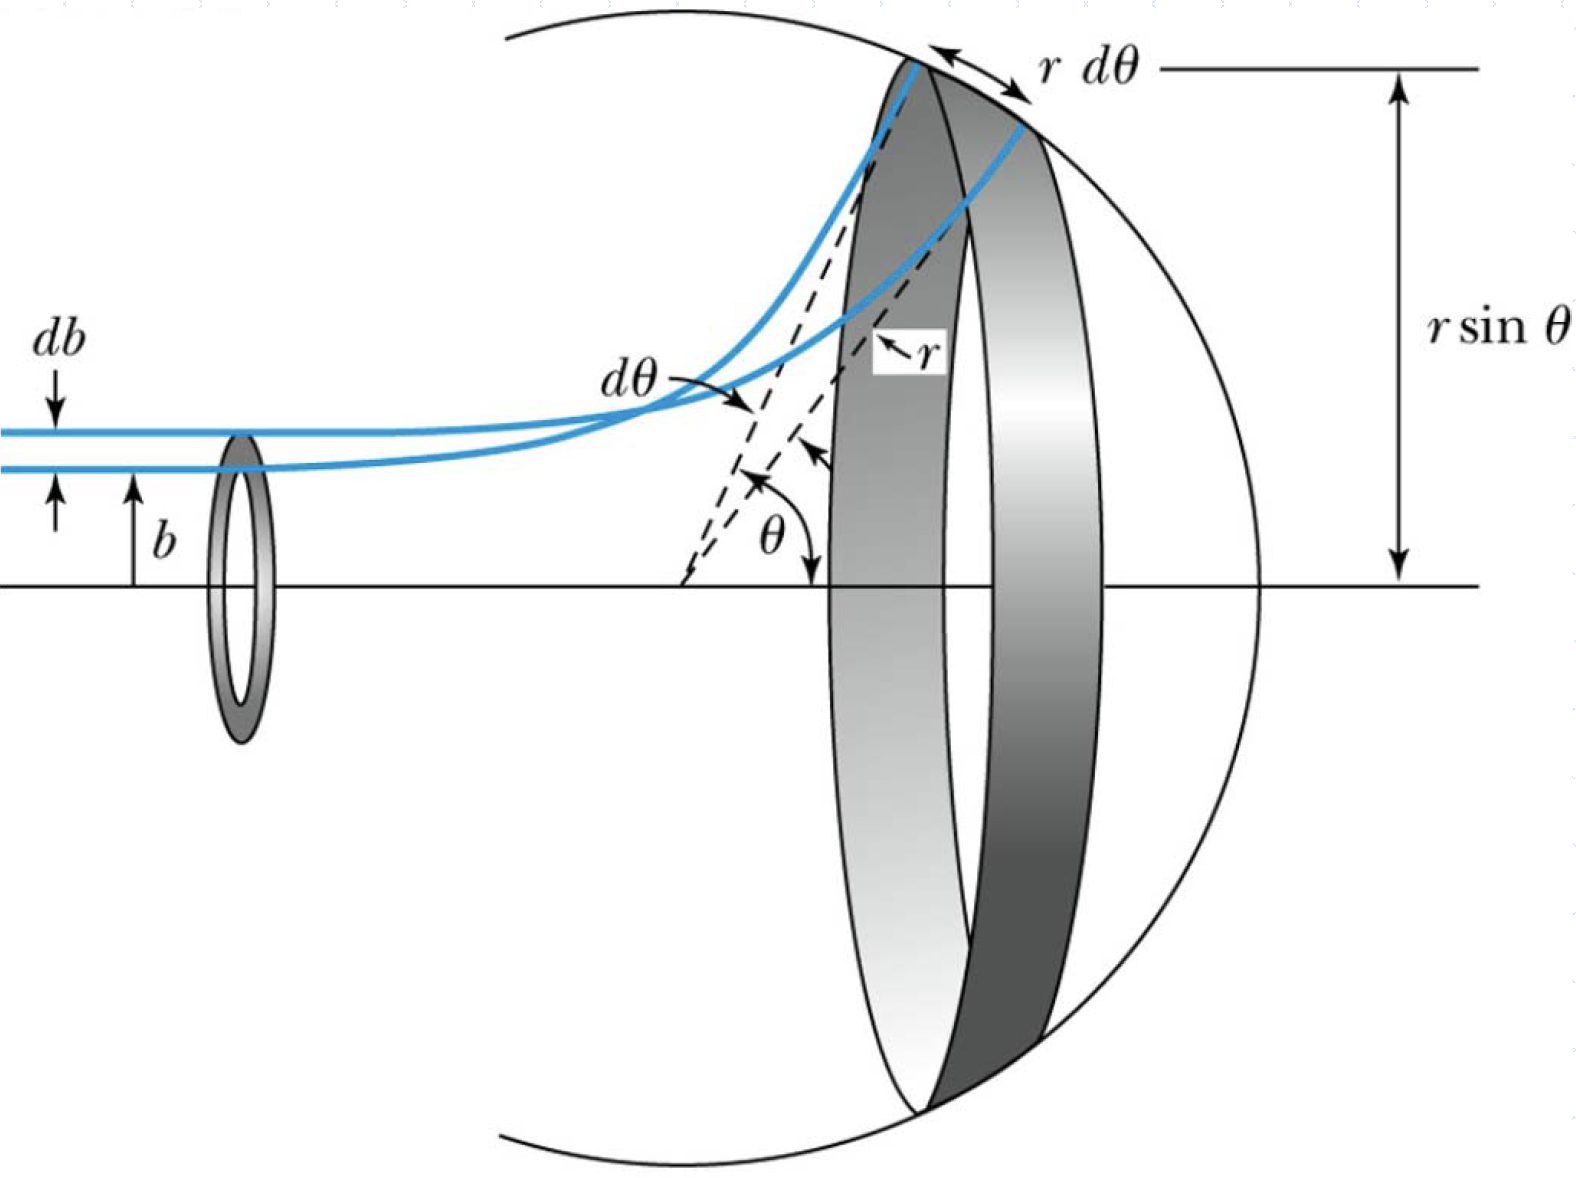
\includegraphics[width=7cm]{src/ScatteringSection.png}
\end{figure}

制备入射粒子束, 保证诸粒子的$E$相同而$b$(从而$J$)不相同. 此时$b$和$\theta$之间会有一一对应. 惟应注意$\brac{b,b+\rd{b}}$对应的$\theta$范围应为$\brac{\theta, \theta-\rd{\theta}}$.
\par
入射时还有入射流强$n$这一参量, 即通过单位时间内单位横截面积的粒子数(粒子数通量).
\begin{flalign*}
    \text{横截面积} && \rd{\theta} &= 2\pi b \,\rd{b}, &\\
    \text{单位时间内入射通量} && \rd{N} &= n\,\rd{\sigma} = 2\pi nb\,\rd{b}. &
\end{flalign*}
由粒子数守恒, $\rd{N} = q\pare{\theta} n\,\rd{\Omega}$. 即单位时间内入射通量等于单位时间内出射通量, 其中
\[ \rd{\Omega} = \sin\theta \rd{\theta} \int_0^{2\pi} \rd{\varphi} = 2\pi \sin\theta\rd{\theta}. \]
而$\displaystyle q\pare{\theta} = \frac{\rd{N}}{n\,\rd{\Omega}} = \+d\Omega d\sigma$谓微分散射截面.
\[ \+d\Omega d\sigma = \frac{2\pi b\,\rd{b}}{2\pi \sin\theta\,\rd{\theta}} = \frac{b}{\sin\theta}\abs{\+d\theta db} = \half\abs{\+d{\cos\theta}d{b^2}} = \rec{4mE} \abs{\+d{\cos\theta}d{J^2}}. \]
若将微分散射截面积分, 则
\[ \sigma_t = \int \pare{\+d\Omega d\sigma}\,\rd{\Omega} = \int\pare{\+d\Omega d\sigma} 2\pi \sin\theta\,\rd{\theta} \]
谓\emph{总散射截面}.

% paragraph 多粒子散射 (end)

\paragraph{钢球散射} % (fold)
\label{par:钢球散射}

对于$\displaystyle V\pare{r} = \begin{cases}
    \infty, & r<R,\\
    0,& r>R
\end{cases}$, 其中$R = r_1 + r_2$是两个刚球的半径和. 根据几何关系立刻有
\[ b = R\sin\varphi_0 = R\cos \frac{\theta}{2}. \]
或者通过定义式
\[ \varphi_0 = \int_{r\+_min_}^\infty \frac{J\,\rd{r}}{r^2 \sqrt{2m\pare{E - V\+_eff_}}}, \]
其中$r\+_min_ = R$, 而有效势为$\displaystyle V\+_eff_ = \frac{J^2}{2mr^2}$, 代入可得
\[ \varphi_0 = \arcsin \pare{\frac{J}{\sqrt{2mE}R}} = \arcsin{\frac{b}{R}}\Rightarrow \cos \frac{\theta}{2} = \cos \pare{\pi - \varphi_0} = \frac{b}{R}. \]
$J^2 = mER^2\pare{1+\cos\theta}$, 得到散射截面
\[ \+d\Omega d\sigma = \rec{4mE}\abs{\+d{\cos\theta}d{J^2}} = \rec{4mE} mER^2 = \frac{R^2}{4}. \]
积分可得总截面为$\pi R^2$. 在实验室系中, $\rd{\sigma_0} = \rd{\sigma}$, $\displaystyle \pare{\frac{\rd{N}}{n}}_0 = \frac{\rd{N}}{n}$, 故
\begin{align*}
    \pare{\+d\Omega d\sigma}_0 &= \+d{\Omega_0}d\sigma = \+d\Omega d\sigma \cdot \+d{\Omega_0}d\Omega \\
    &= \pare{\+d\Omega d\sigma} \frac{\sin\theta\,\rd{\theta}}{\sin\theta_0\,\rd{\theta_0}} = \pare{\+d\Omega d\sigma} \+d{\cos\theta_0}d{\cos\theta}.
\end{align*}
\begin{cenum}
    \item $m_1 \ll m_2$时, $\cos\theta \approx \cos\theta_0 - \frac{\displaystyle}{m_1}{m_2}\sin^2\theta_0 + O\pare{\frac{m_1^2}{m_2^2}}$. 从而
    \[ \pare{\+d\Omega d\sigma}_0 = \pare{\+d\Omega d\sigma}\pare{1+\frac{2m_1}{m_2}\cos\theta_0}. \]
    \item $m_1 = m_2$时, $\theta_0 = \displaystyle \frac{\theta}{2}$, 从而
    \[ \pare{\+d\Omega d\sigma}_0 = 4\cos\theta_0 \pare{\+d\Omega d\sigma}. \]
\end{cenum}

% paragraph 钢球散射 (end)

\paragraph{作业} % (fold)
\label{par:作业}

2.1, 2.2, 2.4, 2.5, 2.6

% paragraph 作业 (end)

% subsubsection 散射的一般理论 (end)

\subsubsection{Rutherford散射} % (fold)
\label{ssub:rutherford散射}

对于$\displaystyle V\pare{r} = \frac{k^2}{r}$, $E>0$,
\begin{align*}
    \varphi &= \pm \int \frac{J\,\rd{r}}{r^2\sqrt{2m\pare{E - \frac{J^2}{2mr^2} + \frac{k^2}{r}}}} \Rightarrow r = \frac{p}{-1 + \epsilon \cos\varphi + C}.\\
    p &= \frac{J^2}{mk^2},\quad \epsilon = \sqrt{1+\frac{2EJ^2}{mk^4}} > 1.
\end{align*}
\begin{remark}
    对于平方反比斥力, 若使入射方向为极轴, 则$C\neq 0$. $C=0$的情况实际如下图(轨道仅取实线的一支). 
    \begin{center}
        \incfig{6cm}{HyperbolaCZero}
    \end{center}
\end{remark}

当$r\rightarrow\infty$, $\epsilon\cos\pare{\varphi+C}\rightarrow 1$, 因此$\varphi+C \rightarrow \pm\displaystyle \arccos \rec{\epsilon}$.
\begin{align*}
    \varphi_1 &= \arccos \rec{\epsilon} - C,\quad \varphi_2 = -\arccos \rec{\epsilon} - C, \\
    2\varphi_0 &= \varphi_1 - \varphi_2 = 2\arccos \rec{\epsilon}\Rightarrow \theta = \pi - 2\varphi_0 = 2 \arcsin \rec{\epsilon.} \\
    \sin \frac{\theta}{2} &= \rec{\epsilon} \Rightarrow \cos \frac{\theta}{2} = \frac{\sqrt{1-\rec{\epsilon^2}}}{1/\epsilon} = \sqrt{\epsilon^2 - 1} = \sqrt{\frac{2EJ^2}{mk^4}}.\\
    \Rightarrow J^2 &= \frac{mk^4}{2E} \frac{1+\cos\theta}{1-\cos\theta}, \\
    \Rightarrow \+d{\cos\theta}d{J^2} &= \frac{mk^4}{E}\rec{\pare{1-\cos\theta}^2} = \frac{mk^4}{4E} \rec{\sin^4\pare{\frac{\theta}{2}}}. \\
    \+d\Omega d\sigma &= \rec{4mE}\abs{\+d{\cos\theta}d{J^2}} = \pare{\frac{k^4}{4E}}^2 \rec{\sin^4 \frac{\theta}{2}}.
\end{align*}
对于Coulomb势, 使用\ce{He}粒子入射, $\displaystyle E = \half mv_\infty^2$,
\[ k^2 = \frac{2e\cdot Ze}{4\pi\omega_0} = \frac{Ze^2}{2\pi \epsilon_0} = \alpha > 0. \]
故在质心系中,
\[ \+d\Omega d\sigma = \frac{\alpha^2}{4m^2v_\infty^4} \rec{\sin^4 \frac{\theta}{2}}. \]
实验室系和质心系的$v_\infty$相同.
\begin{cenum}
    \item $m_1 = m_2$, $m = m_1/2$, $\theta_0 = \theta/2$,
    \[ \pare{\+d\Omega d\sigma}_0 = 4\cos\theta_0 \pare{\+d\Omega d\sigma} = \frac{4\alpha^2}{m_1^2v_\infty^2} \frac{\cos\theta_0}{\sin^4\theta_0}. \]
    \item Rutherford散射的真实情况为$m_1 \ll m_2$, $\displaystyle m \approx m_1 \pare{1-\frac{m_1}{m_2}}$.
    \begin{align*}
        \cos\theta &\approx -\frac{m_1}{m_2}\sin^2\theta_0 + \cos\theta_0 \pare{1-\frac{m_1^2}{2m_2^2}\sin^2\theta_0}, \\
        \sin^{-4}\frac{\theta}{2} &\approx \sin^{-4} \frac{\theta_0}{2}\pare{1-4\frac{m_1}{m_2}\cos^2 \frac{\theta_0}{2}}, \\
        \pare{\+d\Omega d\sigma}_0 &\approx \pare{\+d\Omega d\sigma}\pare{1+\frac{2m_1}{m_2}\cos\theta_0} = \frac{\alpha}{4m_1^2 v_\infty^4}\rec{\sin^4 \frac{\theta_0}{4}}.
    \end{align*}
    即此时实验室系和质心系的散射截面表达式类似.
\end{cenum}
\begin{remark}
    总截面是发散的. 即入射粒子和靶粒子之间的力是长程力.
\end{remark}
\begin{remark}
    在粒子对撞机中, 实验室系和质心系是相同的.
\end{remark}

\paragraph{期中考试} % (fold)
\label{par:期中考试}

11月17日(周日) 下午14:30--17:00, 在5402和5404.

% paragraph 期中考试 (end)

% subsubsection rutherford散射 (end)

% subsection 两体碰撞与散射 (end)

\subsection{多自由度体系的小振动} % (fold)
\label{sub:多自由度体系的小振动}

\subsubsection{简谐振动} % (fold)
\label{ssub:简谐振动}

设简谐振动平衡点位于$x_0=0$, 则$\displaystyle L = \half m\dot{x}^2 - \half kx^2$, $k>0$. 即
\[ m\ddot{x} + kx = 0,\quad \ddot{x} + \omega^2 x = 0. \]
通解为
\begin{align*}
    x &= A_1 \cos\omega t + A_2 \sin\omega t = A\cos\pare{\omega t + \varphi} \\ &= Ce^{i\omega t} + C^* e^{-i\omega t},\quad A_1, A_2, A, \varphi \in \+bR.
\end{align*}
\begin{sample}
    \begin{ex}
        对于单摆, $\displaystyle L = \half ml^2\dot{\theta^2} + mgl\cos\theta$, 平衡点$\theta_0 = 0$,
        \[ L \approx \half ml^2\dot{\theta}^2 + mgl\pare{1-\frac{\theta^2}{2}} = \half ml^2\dot{\theta}^2 - \half mgl\theta^2 + \cancelto{}{mgl}. \]
        得到运动方程
        \[ \ddot{\theta} + \frac{g}{l}\sin\theta = 0,\quad \ddot{\theta} + \frac{g}{l}\theta = 0,\quad \omega = \sqrt{\frac{g}{l}}. \]
    \end{ex}
\end{sample}
\begin{figure}[ht]
    \centering
    \incfig{8cm}{CoupledPendulum}
    \caption{耦合摆}
    \label{fig:耦合摆}
\end{figure}
\begin{sample}
    \begin{ex}[耦合摆]
        \label{ex:耦合摆}
        如\cref{fig:耦合摆}, 平衡点$\theta_{10} = 0$, $\theta_{20} = 0$, 弹簧自然长度$a$. 设$\abs{\theta_1}, \abs{\theta_2}\ll 1$, 则
        \begin{align}
            T &= \half ml^2\pare{\dot{\theta}_1^2 + \dot{\theta}_2^2}, \notag\\
            V_g &= -mgl\pare{\cos\theta_1 + \cos\theta_2} \approx \half mgl\pare{\theta_1^2 + \theta_2^2} - 2mgl, \notag\\
            V_k &= \half k \Delta^2 = \half k\brac{2l^2 - 2l^2 \cos\pare{\theta_2 - \theta_1}}\notag\\
            &= kl^2 \brac{1-\cos\pare{\theta_2 - \theta_1}} \notag\\
            &\approx \half kl^2 \pare{\theta_2 - \theta_1}^2.\notag\\
            L &= T-V = \half ml^2\pare{\dot{\theta}_1^2 + \dot{\theta}_2^2} - \half mgl\pare{\theta_1^2 + \theta_2^2} - \half kl^2\pare{\theta_2 - \theta_1}^2.\notag\\
            \label{eq:耦合摆1}
            &\+dtd{}\+D{\dot{\theta}_1}DL = \+D{\theta_1}DL \Rightarrow ml\ddot{\theta}_1 + \pare{mg+kl}\theta_1 - kl\theta_2 = 0, \\
            \label{eq:耦合摆2}
            &\+dtd{}\+D{\dot{\theta}_2}DL = \+D{\theta_2}DL \Rightarrow ml\ddot{\theta}_2 - kl\theta_1 + \pare{mg+kl}\theta_2 = 0.
        \end{align}
    \end{ex}
\end{sample}
欲求解上述方程, 使用试探解
\[ \left\{\begin{aligned}
    \theta_1 &= A\sin\pare{\omega t + \varphi_0}, \\
    \theta_2 &= B\sin\pare{\omega t + \varphi_0}.
\end{aligned}\right. \]
其中$A,B,\omega$待定. 代入可得
\begin{align*}
    \pare{-ml\omega^2+mg+kl} \theta_1 - kl\theta_2 &= 0, \\
    -kl\theta_1 + \pare{-ml\omega^2 + mg + kl}\theta_2 &= 0.
\end{align*}
如果分别除以$\sin\pare{\omega t + \varphi_0}$, 有
\begin{align*}
    \pare{-ml\omega^2+mg+kl} A - kl B &= 0, \\
    -klA + \pare{-ml\omega^2 + mg + kl} B &= 0.
\end{align*}
这是关于$A, B$的方程组. 欲使得方程有非零振幅解, 必有
\begin{align*}
    & \begin{vmatrix}
    {-ml\omega^2+mg+kl} & - kl \\
    -kl & {-ml\omega^2 + mg + kl}
\end{vmatrix} = 0 \\ &\Rightarrow {-ml\omega^2+mg+kl} = \pm kl \Rightarrow \omega_1^2 = \frac{g}{l},\quad \omega_2^2 = \frac{g}{l}+\frac{2k}{m} \\
&\Rightarrow \omega_1 = \sqrt{\frac{g}{l}},\quad \omega_2 = \sqrt{\frac{g}{l} + \frac{2k}{m}}.
\end{align*}
\begin{cenum}
    \item $\omega = \omega_1$, 此时
    \begin{align*}
        & \begin{pmatrix}
        kl & -kl \\ -kl & kl
    \end{pmatrix} \begin{pmatrix}
        A \\ B
    \end{pmatrix} = 0 \\ &\Rightarrow A = B = A_1,\quad \theta_1^{\pare{1}} = A_1\sin\pare{\omega_1 t + \varphi_0^{\pare{1}}} = \theta_2^{\pare{1}}.
    \end{align*}
    \item $\omega = \omega_2$, 此时
    \begin{align*}
        & \begin{pmatrix}
        -kl & -kl \\
        -kl & -kl
    \end{pmatrix} \begin{pmatrix}
        A \\ B
    \end{pmatrix} = 0 \\ &\Rightarrow A = -B = A_2,\quad \theta_1^{\pare{2}} = A_2\sin\pare{\omega_2 t + \varphi_0^{\pare{2}}} = -\theta_2^{\pare{2}}.
    \end{align*}
\end{cenum}
通解
\begin{align*}
    \theta_1 &= \theta_1^{\pare{1}} + \theta_1^{\pare{2}} = A_1\sin\pare{\omega_1 t + \varphi_0^{\pare{1}}} + A_2\sin\pare{\omega_2 t + \varphi_0^{\pare{2}}}, \\
    \theta_2 &= \theta_2^{\pare{1}} + \theta_2^{\pare{2}} = A_1\sin\pare{\omega_1 t + \varphi_0^{\pare{1}}} - A_2\sin\pare{\omega_2 t + \varphi_0^{\pare{2}}}.
\end{align*}
也可以引入简正坐标
\begin{align*}
    \xi_1 &= \theta_1 + \theta_2 = 2\theta_1^{\pare{1}} = 2A_1 \sin\pare{\omega_1 t + \varphi_1^{\pare{0}}}, \\
    \xi_2 &= \theta_1 - \theta_2 = 2\theta_1^{\pare{2}} = 2A_2 \sin\pare{\omega_2 t + \varphi_2^{\pare{0}}}.
\end{align*}
故$\xi_1$和$\xi_2$分别以两种独立的振动模式振动. 通过
\[ \theta_1 = \half\pare{\xi_1 + \xi_2},\quad \theta_2 = \half\pare{\xi_1 - \xi_2} \]
逆变换得到$\theta_1$和$\theta_2$.
\par
\begin{figure}[ht]
    \centering
    \begin{subfigure}{5cm}
        \centering
        \incfig{4.5cm}{CoupledPendulumS1}
        \caption{}
        \label{fig:第一种简正模式}
    \end{subfigure}
    \begin{subfigure}{5cm}
        \centering
        \incfig{4.5cm}{CoupledPendulumS2}
        \caption{}
        \label{fig:第二种简正模式}
    \end{subfigure}
    \caption{}
\end{figure}
在简正模式下, 仅在一个频率发生振动,
\begin{cenum}
    \item $\xi_1 \neq 0$, $\xi_2 = 0$. 这可以通过$\theta_1\pare{0} = \theta_2\pare{0}$, $\dot{\theta}_1\pare{0} = \dot{\theta}_2\pare{0} = 0$保证. 此时两个摆发生同步振动(如\cref{fig:第一种简正模式}), $\omega = \omega_1 = \displaystyle \sqrt{\frac{g}{l}}$.
    \item $\xi_1 = 0$, $\xi_2 \neq 0$, 这可以通过$\theta_1\pare{0} = -\theta_2\pare{0}$, $\dot{\theta}_1\pare{0} = \dot{\theta}_2\pare{0} = 0$保证. 此时两个摆发生异步振动(如\cref{fig:第二种简正模式}), $\omega = \omega_2 = \displaystyle \sqrt{\frac{g}{l} + \frac{2k}{m}}$.
\end{cenum}
\par
另一种求解\cref{ex:耦合摆}中的方程的方法谓考虑两个方程之和与差,
\begin{flalign*}
    \eqref{eq:耦合摆1} + \eqref{eq:耦合摆2} && ml\pare{\ddot{\theta}_1 + \ddot{\theta}_2} + mg\pare{\theta_1 + \theta_2} &= 0, &\\
    \eqref{eq:耦合摆1} - \eqref{eq:耦合摆2} && ml\pare{\ddot{\theta}_1 - \ddot{\theta}_2} + \pare{mg+2kl}\pare{\theta_1 - \theta_2} &= 0. &
\end{flalign*}
令$\xi_1 = \theta_1 + \theta_2$, $\xi_2 = \theta_1 - \theta_2$, 得到
\begin{align*}
    ml\ddot{\xi}_1 + mg\xi_1 &= 0, \\
    ml\ddot{\xi}_2 + \pare{mg+2kl} \xi_2 &= 0.
\end{align*}
\par
还有一种求解\cref{ex:耦合摆}中的方程的方法谓配方, 即
\begin{align*}
    T &= \half ml^2 \pare{\dot{\theta}_1^2 + \dot{\theta}_2^2} \\
    &= \rec{4} ml^2\brac{\pare{\dot{\theta}_1+\dot{\theta}_2}^2 + \pare{\dot{\theta}_1 - \dot{\theta}_2}^2} \\
    &= \rec{4} ml^2\pare{\xi_1^2 + \xi_2^2}. \\
    V &= \half mgl\pare{\theta_1^2 + \theta_2^2} + \half kl^2 \pare{\theta_1 - \theta_2}^2 \\
    &= \rec{4} mgl\brac{\pare{\theta_1 + \theta_2}^2 + \pare{\theta_1 - \theta_2}^2} + \half kl^2 \pare{\theta_1 - \theta_2}^2 \\
    &= \rec{4} mgl\pare{\xi_1^2 + \xi_2^2} + \half kl^2 \xi_2^2. \\
    L &= \rec{4}ml^2\pare{\dot{\xi}_1^2 + \dot{\xi}_2^2} - \rec{4}mgl\xi_1^2 - \rec{4}\pare{mgl+2kl^2}\xi_2^2 \\
    &= \rec{4}ml^2 \dot{\xi}_1^2 - \rec{4}mgl\xi_1^2 + \rec{4}ml^2\dot{\xi}_2^2 - \rec{4}\pare{mgl + 2kl^2}\xi_2^2.
\end{align*}
此时$\xi_1$和$\xi_2$完全分离, 故分别构成两个简正模.
\par
也可以通过矩阵对角化之手段求解之.
\[ \underbrace{\begin{pmatrix}
    ml & 0 \\ 0 & ml
\end{pmatrix}}_{\+vM}\begin{pmatrix}
    \ddot{\theta}_1 \\ \ddot{\theta}_2
\end{pmatrix} + \underbrace{\begin{pmatrix}
    mg+kl & -kl \\ -kl & mg+kl
\end{pmatrix}}_{\+vK}\begin{pmatrix}
    \theta_1 \\ \theta_2
\end{pmatrix} = 0. \]
其中$\+vM$和$\+vK$都是实对称矩阵. 方程可以写为
\[ \begin{pmatrix}
    \ddot{\theta}_1 \\ \ddot{\theta}_2
\end{pmatrix} + \+vM^{-1}\+vK \begin{pmatrix}
    \theta_1 \\ \theta_2
\end{pmatrix} = 0,\quad \+vM^{-1}\+vK = \begin{pmatrix}
    g/l + k/m & -k/m \\
    -k/m & g/l + k/m
\end{pmatrix}. \]
考虑一线性变换
\[ \begin{pmatrix}
    \theta_1 \\
    \theta_2
\end{pmatrix} = \+vA \begin{pmatrix}
    \xi_1 \\
    \xi_2
\end{pmatrix}\Leftrightarrow \begin{pmatrix}
    \xi_1 \\
    \xi_2
\end{pmatrix} = \+vA^{-1}\begin{pmatrix}
    \theta_1 \\
    \theta_2
\end{pmatrix}. \]
其中$\+vA$可逆. 则
\[ \begin{pmatrix}
    \ddot{\xi}_1 \\ \ddot{\xi}_2
\end{pmatrix} = \+vA^{-1} \begin{pmatrix}
    \ddot{\theta}_1 \\ \ddot{\theta}_2
\end{pmatrix} = -\+vA^{-1}\+vM^{-1}\+vK \begin{pmatrix}
    \theta_1\\\theta_2
\end{pmatrix} = -\+vA^{-1} \+vM^{-1}\+vK\+vA \begin{pmatrix}
    \xi_1 \\
    \xi_2
\end{pmatrix}. \]
如果
\[ \+v\Omega = \+vA^{-1}\pare{\+vM^{-1}\+vK}\+vA = \begin{pmatrix}
    \lambda_1 & 0 \\
    0 & \lambda_2
\end{pmatrix} \]
是对角矩阵, 则有
\[ \begin{cases}
    \ddot{\xi}_1 + \lambda_1 \xi_1 &= 0, \\
    \ddot{\xi}_2 + \lambda_2 \xi_2 &= 0
\end{cases}\Rightarrow \begin{cases}
    \xi_1 &= A_1 \sin\pare{\sqrt{\lambda_1} t + \varphi_0^{\pare{0}}}, \\
    \xi_2 &= A_2 \sin\pare{\sqrt{\lambda_2} t + \varphi_0^{\pare{1}}}.
\end{cases} \]
现在问题被转化为了本征值问题,
\begin{align*}
    \+vM^{-1}\+vK \begin{pmatrix}
    x_1 \\ x_2
\end{pmatrix} &= \lambda \begin{pmatrix}
    x_1 \\ x_2
\end{pmatrix} \\
\Rightarrow \pare{\+vM^{-1}\+vK - \lambda\+vE} \begin{pmatrix}
    x_1 \\ x_2
\end{pmatrix} &= 0. \\
\pare{\+vK - \lambda\+vM} \begin{pmatrix}
    x_1 \\ x_2
\end{pmatrix} &= 0.
\end{align*}
欲使之有非零解, 须
\begin{align*}
    \det \pare{\+vK - \lambda \+vM} = 0 &\Rightarrow \begin{vmatrix}
    mg + kl - \lambda ml & -kl \\
    -kl & mg + kl - \lambda ml
    \end{vmatrix} = 0. \\
    mg + kl - \lambda ml &= \pm kl \Rightarrow \lambda_1 = \frac{g}{l},\quad \lambda_2 = \frac{g}{l} + \frac{2k}{m}. \\
    \lambda = \lambda_1 \Rightarrow \begin{pmatrix}
        kl & -kl \\ -kl & kl
    \end{pmatrix} \begin{pmatrix}
        x_1^{\pare{1}} \\ x_2^{\pare{2}}
    \end{pmatrix} &= 0 \Rightarrow x_1^{\pare{1}} = x_2^{\pare{2}} \Rightarrow \begin{pmatrix}
        x_1^{\pare{1}} \\ x_2^{\pare{2}}
    \end{pmatrix} = \mu_1 \begin{pmatrix}
        1 \\ 1
    \end{pmatrix}. \\
    \lambda = \lambda_2 \Rightarrow \begin{pmatrix}
        -kl & -kl \\ -kl & -kl
    \end{pmatrix} \begin{pmatrix}
        x_1^{\pare{1}} \\ x_2^{\pare{2}}
    \end{pmatrix} &= 0 \Rightarrow x_1^{\pare{1}} = -x_2^{\pare{2}} \Rightarrow \begin{pmatrix}
        x_1^{\pare{1}} \\ x_2^{\pare{2}}
    \end{pmatrix} = \mu_2 \begin{pmatrix}
        1 \\ -1
    \end{pmatrix}.
\end{align*}
先证明不同本征值的本征矢量是相互正交的.
\begin{align*}
    \+vK \ket{x^{\pare{i}}} = \lambda_i \+vM \ket{x^{\pare{i}}} &\Rightarrow \bra{x^{\pare{i}}} \+vK^T = \lambda_i \bra{x^{\pare{i}}} \+vM^T\\ &\Rightarrow \bra{x^{\pare{i}}} \+vK = \lambda_i \bra{x^{\pare{i}}} \+vM. \\
    \bra{x^{\pare{j}}} \+vK \ket{x^{\pare{i}}} &= \lambda_i \bra{x^{\pare{j}}} \+vM \ket{x^{\pare{i}}}. \\
    &= \lambda_j \bra{x^{\pare{j}}} \+vM \ket{x^{\pare{i}}}. \\
    \lambda_i \neq \lambda_j &\Rightarrow \bra{x^{\pare{j}}} \+vM \ket{x^{\pare{i}}} = 0.
\end{align*}
若人为要求$\bra{x^{\pare{i}}}\+vM \ket{x^{\pare{i}}} = 1$, 则可以让诸$x^{\pare{i}}$满足规范正交性
\[ \bra{x^{\pare{i}}}\+vM \ket{x^{\pare{j}}} = \delta_{ij}. \]
构造
\[ \+vA = \begin{pmatrix}
    x_1^{\pare{1}} & x_1^{\pare{2}} \\
    x_2^{\pare{1}} & x_2^{\pare{2}}
\end{pmatrix} = \begin{pmatrix}
    \mu_1 & \mu_2 \\
    \mu_1 & -\mu_2
\end{pmatrix},\quad \+vA^T = \begin{pmatrix}
    x_1^{\pare{1}} & x_2^{\pare{1}} \\
    x_1^{\pare{2}} & x_2^{\pare{2}}
\end{pmatrix} = \begin{pmatrix}
    \mu_1 & \mu_1 \\
    \mu_2 & -\mu_2
\end{pmatrix}. \]
则
\begin{align*}
    \+vA^T \+vM \+vA &= \bra{x^{\pare{1}}, x^{\pare{2}}} \+vM \ket{x^{\pare{1}},x^{\pare{2}}} = \+vE\Rightarrow \+vA^T = \pare{\+vM\+vA}^{-1} = \+vA^{-1}\+vM^{-1}. \\
    \+v\Omega &= \+vA^{-1}\+vM\+vK\+vA = \pare{\+vA^{-1}\+vM^{-1}}\+vK\+vA = \+vA^T \+vK\+vA \\
    &= \bra{x^{\pare{1}}, x^{\pare{2}}} \+vK \ket{x^{\pare{1}},x^{\pare{2}}} \\
    &= \bra{x^{\pare{1}}, x^{\pare{2}}} \+vM \ket{\lambda_1 x^{\pare{1}},\lambda_2 x^{\pare{2}}} \\
    &= \begin{pmatrix}
        \lambda_1 & 0 \\
        0 & \lambda_2
    \end{pmatrix}. \\
    \begin{pmatrix}
        \xi_1 \\ \xi_2
    \end{pmatrix} &= \+vA^{-1}\begin{pmatrix}
        \theta_1 \\ \theta_2
    \end{pmatrix} = \+vA^T \+vM \begin{pmatrix}
        \theta_1 \\ \theta_2
    \end{pmatrix} = \begin{pmatrix}
        \mu_1 \mu_1 \\ \mu_2 -\mu_2
    \end{pmatrix}\begin{pmatrix}
        ml & 0 \\
        0 & ml
    \end{pmatrix}\begin{pmatrix}
        \theta_1 \\ \theta_2
    \end{pmatrix} \\ &= ml \begin{pmatrix}
        \mu_1 & \mu_1 \\
        \mu_2 & -\mu_2
    \end{pmatrix}\begin{pmatrix}
        \theta_1 \\ \theta_2
    \end{pmatrix} = \begin{pmatrix}
        ml\mu_1\pare{\theta_1 + \theta_2} \\
        ml\mu_2\pare{\theta_1 - \theta_2}
    \end{pmatrix}.
\end{align*}

\paragraph{作业} % (fold)
\label{par:作业}

2.9, 2.10, 2.11, 2.12

% paragraph 作业 (end)

\begin{figure}[ht]
    \centering
    \incfig{6cm}{GenCoor2}
\end{figure}
\begin{figure}[ht]
    \centering
    \begin{subfigure}{5cm}
        \centering
        \incfig{5cm}{GenCoor2Mode1}
        \caption{}
        \label{fig:双摆简正模式1}
    \end{subfigure}
    \begin{subfigure}{5cm}
        \centering
        \incfig{5cm}{GenCoor2Mode2}
        \caption{}
        \label{fig:双摆简正模式2}
    \end{subfigure}
    \caption{}
\end{figure}
\begin{sample}
    \begin{ex}
        对于双摆系统,
        \begin{align*}
            &\begin{cases}
            x_2 &= l\pare{\sin\theta_1 + \sin\theta_2}, \\
            y_2 &= l\pare{\cos\theta_1 + \cos\theta_2}.
            \end{cases}\\
            T_1 &= \half ml^2\dot{\theta}_1^2, \\
            T_2 &= \half m\pare{\dot{x}_2^2 + \dot{y}_2^2} \\
            &= \half ml^2 \brac{\dot{\theta}_1^2 + \dot{\theta}_2^2 + 2\dot{\theta}_1\dot{\theta}_2\cos\pare{\theta_1 - \theta_2}} \\
            &= \half m l^2 \brac{\dot{\theta}_1^2 + \dot{\theta}_2^2 + 2\dot{\theta}_1\dot{\theta}_2} = \half ml^2\pare{\dot{\theta}_1 + \dot{\theta}_2}^2.
        \end{align*}
        其中$\abs{\theta_1} \ll 1$, $\abs{\theta_2}\ll 2$, 故可以假设$\dot{\theta}_1$和$\dot{\theta}_2$也是同阶的小量.
        \begin{align*}
            V &= -mgl\cos\theta_1 - mgl \pare{\cos\theta_1 + \cos\theta_2} \\
            &\approx mgl\pare{\theta_1^2 + \half \theta_2^2} - 3mgl. \\
            L &= T-V  = T_1 + T_2 - V \\
            &= \half ml^2\pare{2\dot{\theta}_1^2 + 2\dot{\theta}_1\dot{\theta}_2 + \dot{\theta}_2^2} - mgl\pare{\theta_1^2 + \half \theta_2^2}. \\
            \+D{\theta_i}DL &= \+dtd{} \+D{\dot{\theta}_i}DL = 0. \\
            &\begin{cases}
                ml^2 \pare{2\ddot{\theta}_1 + \ddot{\theta}_2} + 2mgl\theta_1 &= 0, \\
                ml^2 \pare{\ddot{\theta}_1 + \ddot{\theta}_2} + mgl\theta_2 &= 0.
            \end{cases} \\
            & \underbrace{\begin{pmatrix}
                2 & 1 \\
                1 & 1
            \end{pmatrix}}_{\+vM}\begin{pmatrix}
                \ddot{\theta}_1 \\
                \ddot{\theta}_2
            \end{pmatrix} + \frac{g}{l} \underbrace{\begin{pmatrix}
                2 & 0 \\ 0 & 1
            \end{pmatrix}}_{\+vK}\begin{pmatrix}
                \theta_1 \\ \theta_2
            \end{pmatrix} = 0. \\
            \begin{pmatrix}
                \theta_1 \\ \theta_2
            \end{pmatrix} &= \+vA \begin{pmatrix}
                \xi_1 \\ \xi_2
            \end{pmatrix},\quad \begin{pmatrix}
                \xi_1 \\ \xi_2
            \end{pmatrix} = \+vA^{-1}\begin{pmatrix}
                \theta_1 \\ \theta_2
            \end{pmatrix}. \\
            & \begin{pmatrix}
                \ddot{\xi}_1 \\ \ddot{\xi}_2
            \end{pmatrix} + \+vA^{-1}\pare{\+vM^{-1}\+vK}\+vA \begin{pmatrix}
                \xi_1 \\ \xi_2
            \end{pmatrix} = 0. \\
            & \det{\+vK - \lambda \+vM} = 0 \Rightarrow \begin{vmatrix}
                2g/l - 2\lambda & -\lambda \\ -\lambda & g/l - \lambda
            \end{vmatrix} = 0. \\
            \lambda &= \lambda_1 = \pare{2\sqrt{2}}g/l\Rightarrow \begin{pmatrix}
                x_1^{\pare{1}} \\ x_2^{\pare{1}}
            \end{pmatrix} = \mu_1 \begin{pmatrix}
                1 \\ \sqrt{2}
            \end{pmatrix}, \\
            \lambda &= \lambda_2 = \pare{2+\sqrt{2}}g/l \Rightarrow \begin{pmatrix}
                x_1^{\pare{2}} \\ x_2^{\pare{2}}
            \end{pmatrix} = \mu_2 \begin{pmatrix}
                1 \\ -\sqrt{2}
            \end{pmatrix}. \\
            &\begin{pmatrix}
                x_1^{\pare{i}} & x_2^{\pare{i}}
            \end{pmatrix} \+vM \begin{pmatrix}
                x_1^{\pare{j}} \\ x_2^{\pare{j}}
            \end{pmatrix} = \delta_{ij} \Rightarrow \+vA^T \+vM\+vA = \+vE. \\
            &\+vA^{-1} = \+vA^T \+vM = \begin{pmatrix}
                \pare{2+\sqrt{2}} \mu_1 & \sqrt{1+\sqrt{2}}\mu_1 \\
                \pare{2-\sqrt{2}}\mu_2 & \sqrt{1-\sqrt{2}} \mu_2
            \end{pmatrix} \\ &\Rightarrow \begin{cases}
                \ddot{\xi}_1 + \sqrt{2-\sqrt{2}} \cdot \frac{g}{l} \xi_1 &= 0, \\
                \ddot{\xi}_2 + \sqrt{2+\sqrt{2}} \cdot \frac{g}{l} \xi_2 &= 0.
            \end{cases}\\
            & \begin{pmatrix}
                \xi_1 \\ \xi_2
            \end{pmatrix} = \+vA^{-1} \begin{pmatrix}
                \theta_1 \\ \theta_2
            \end{pmatrix} \Rightarrow \begin{cases}
                \xi_1 &= \pare{1+\sqrt{2}} \mu_1\pare{\sqrt{2}\theta_1 + \theta_2}, \\
                \xi_2 &= \pare{\sqrt{2}-1} \mu_1\pare{\sqrt{2}\theta_1 - \theta_2}.
            \end{cases}
        \end{align*}
        简正模式为
        \begin{cenum}
            \item $\xi_1 \neq 0, \xi_2 = 0$, $\sqrt{2}\theta_1 = \theta_2$, 即两个摆同相位摆动, 如\cref{fig:双摆简正模式1}.
            \item $\xi_1 = 0, \xi_2 \neq 0$, $\theta_2 = -\sqrt{2}\theta_1$, 即两个摆反相位摆动, 如\cref{fig:双摆简正模式2}.
        \end{cenum}
    \end{ex}
\end{sample}
\begin{figure}[ht]
    \centering
    \incfig{6cm}{Trimole}
    \caption{三原子分子振动}
    \label{fig:三原子分子振动}
\end{figure}
\begin{figure}[ht]
    \centering
    \begin{subfigure}{6cm}
        \incfig{6cm}{TrimoleVert}
        \caption{横向振动的情形}
        \label{fig:横向振动的情形}
    \end{subfigure}
    \caption{}
\end{figure}
\begin{figure}[ht]
    \centering
    \begin{subfigure}{6cm}
        \centering
        \incfig{6cm}{TrimoleMode1}
        \caption{}
        \label{fig:三原子分子简正模式1}
    \end{subfigure}
    \begin{subfigure}{6cm}
        \centering
        \incfig{6cm}{TrimoleMode2}
        \caption{}
        \label{fig:三原子分子简正模式2}
    \end{subfigure}
    \caption{}
\end{figure}
\begin{sample}
    \begin{ex}[三原子分子振动]
        考虑如\cref{fig:三原子分子振动}的分子, 振动自由度为
        \[ 3\times 3 - \underbrace{3}_{\text{平动}} - \underbrace{2}_{\text{转动}} = \underbrace{4}_{\text{振动}} = \underbrace{2}_{\text{纵向}}+\underbrace{2}_{\text{横向}}. \]
        平衡位置在$A\pare{-x_0,0,0}$, $B\pare{0,0,0}$, $A\pare{x_0,0,0}$, 其中$B$恰为质心. 横向振动(如\cref{fig:横向振动的情形})只需要分析$x$-$y$平面内的振动($x$-$z$平面内类似). 由条件和动量与角动量守恒, 有
        \begin{align*}
            z_1 &= z_2 = z_3 = 0, \\
            x_1 &= -x_0,\quad x_2 = 0,\quad x_3 = x_0, \\
            y_C &= 0 \Rightarrow m\pare{y_1+y_3} + My_2 = 0 \Rightarrow y_2 = -\frac{m}{M}\pare{y_1+y_3}, \\
            J_z &= 0 \Rightarrow mx_1\dot{y_1} + Mx_2\dot{y_2} + mx_3\dot{y}_3 = mx_0 \pare{\dot{y}_3 - \dot{y}_1} = 0 \Rightarrow y_1 = y_3.
        \end{align*}
        因此$y$方向的振动仅有一个自由度, 取$y_2$为广义坐标, $\displaystyle y_1 = y_3 = -\frac{M}{2m}y_2$.
        \begin{align*}
            T &= \half m\pare{\dot{y}_1^2 + \dot{y}_3^2} + \half M\dot{y}_2^2 = \frac{M}{2}\pare{\frac{M}{2m}+1}\dot{y}_2^2. \\
            V &= V\pare{y_2} = V\pare{0} + \left.\+d{y_2}dV\right\vert_{0}y_2 + \half \left.\frac{\rd{^2V}}{\rd{y_2^2}}\right\vert_{0} y_2^2 + \cdots = \half k'y_2^2. \\
            L &= T-V = \half M\pare{\frac{M}{2m}+1}\dot{y}_2^2 - \half k' y_2^2 \\
            &= \half M'\dot{y}_2^2 - \half k' y_2^2. \\
            0 &= \ddot{y}_2 + \frac{k'}{M'}y_2 \Rightarrow y_2 = A\sin\pare{\sqrt{\frac{k'}{M'}}t + \varphi_0},\quad \omega_{\perp} = \sqrt{\frac{k'}{M'}}.
        \end{align*}
        对于纵向振动, $y_i = 0, z_i = 0$, $i = 1,2,3$.
        \begin{align*}
            T &= \half m\pare{\dot{x}_1^2 + \dot{x}_3^2} - \half M\dot{x}_2^2.
        \end{align*}
        质心不动, 故
        \[ m\pare{x_1+x_3} + Mx_2 = 0. \]
        纵向振动时, 独立广义坐标有两个, 选为$x_1$和$x_3$. 势能
        \[ V = \half k\brac{\pare{x_2-x_1-x_0}^2 + \pare{x_3-x_2-x_0}^2}. \]
        在平衡位置, $x_1 = -x_0$, $x_2=  0$, $x_3 = x_0$. 设
        \begin{align*}
            \overbar{x}_1 &= x_1 + x_0, \Rightarrow \dot{\overbar{x}}_1 = \dot{x}_1, \\
            \overbar{x}_3 &= x_3 - x_0, \Rightarrow \dot{\overbar{x}}_3 = \dot{x}_3, \\
            \overbar{x}_2 &= x_2, \Rightarrow \overbar{x}_2 = -\frac{m}{M}\pare{\overbar{x}_1 + \overbar{x}_3}. \\
            T&= \half m \pare{\dot{\overbar{x}}_1^2 + \dot{\overbar{x}}_3^2} + \frac{m^2}{2M}\pare{\dot{\overbar{x}}_1 + \dot{\overbar{x}}_3}^2, \\
            V&= \half k \brac{\pare{\overbar{x}_2 - \overbar{x}_1}^2 + \pare{\overbar{x}_3 - \overbar{x}_2}^2} \\
            &= \half k \brac{\frac{2m}{M}\pare{1+\frac{m}{M}} \pare{\overbar{x}_1 + \overbar{x}_3}^2 + \overbar{x}_1^2 + \overbar{x}_3^2}. \\
            L &= T-V = \frac{m}{4} \brac{\pare{\dot{\overbar{x}}_1 + \dot{\overbar{x}}_3}^2 + \pare{\dot{\overbar{x}}_1 - \dot{\overbar{x}}_3}^2} + \frac{m^2}{2M}\pare{\dot{\overbar{x}}_1 + \dot{\overbar{x}}_3}^2 \\
            &\phantom{=}\ -\frac{km}{2}\pare{\frac{m}{M}+1}\pare{\overbar{x}_1 + \overbar{x}_3}^2 - \frac{k}{4}\brac{\pare{\overbar{x}_1 + \overbar{x}_3}^2 + \pare{\overbar{x}_1 - \overbar{x}_3}^2}. \\
            \xi_1 &= \overbar{x}_1 + \overbar{x}_3 = x_1 + x_3,\quad \xi_2 = \overbar{x}_1 - \overbar{x}_3 = x_1 - x_3 + 2x_0, \\
            L &= \half m\pare{\half + \frac{m}{M}}\dot{\xi}_1^2 + \frac{m}{4} \dot{\xi}_2^2 - k\pare{\half + \frac{m}{M}}^2 \xi_1^2 - \frac{k}{4}\xi_2^2. \\
            & m\ddot{\xi}_1 + 2k\pare{\half + \frac{m}{M}} \xi_1 = 0\Rightarrow \omega_1^2 = \frac{k}{m} + \frac{2k}{M}, \\
            & m\ddot{\xi}_2 + k\xi_2 = 0 \Rightarrow \omega_2^2 = \frac{k}{m}.
        \end{align*}
        简正模式为
        \begin{cenum}
            \item $\xi_1 \neq 0, \xi_2 = 0$, $\overbar{x}_1 = \overbar{x}_3$, $\displaystyle \overbar{x}_2 = -\frac{2m}{M}\overbar{x}_1$, $\omega = \omega_1$(如\cref{fig:三原子分子简正模式1}).
            \item $\xi_1 = 0, \xi_2\neq 0$, $\overbar{x}_1 = -\overbar{x}_3, \overbar{x}_2 = x_2 = 0$, $\displaystyle \omega = \omega_2 = \sqrt{\frac{k}{m}}$(如\cref{fig:三原子分子简正模式2}).
        \end{cenum}
    \end{ex}
\end{sample}

% subsubsection 简谐振动 (end)

\subsubsection{\texorpdfstring{$S$}{S}个自由度的小振动} % (fold)
\label{ssub:s个自由度的小振动}

平衡位形于$q_{\alpha_0} = 0$, 在平衡位形附近
\begin{align*}
    V\pare{q_\alpha} &= \cancelto{}{V\pare{0}} + \sum_{\alpha=1}^s \cancelto{0}{\left. \+D{q_\alpha}DV \right\vert_0} q_\alpha + \half\sum_{\alpha,\beta=1}^s \left. \frac{\partial^2 V}{\partial q_\alpha \partial q_\beta} \right\vert_0 q_\alpha q_\beta + \cdots \\
    &\approx \half\sum_{\alpha,\beta=1}^s \left. \frac{\partial^2 V}{\partial q_\alpha \partial q_\beta} \right\vert_0 q_\alpha q_\beta \\
    &= \half \sum_{\alpha,beta} k_{\alpha,\beta} q_\alpha q_\beta.
\end{align*}
为使平衡稳定, 须$\+vK$构成一正定矩阵. 对于定常约束,
\begin{align*}
    T &= \cancelto{}{T_0 + T_1} + T_2, \\
    T &= \half \sum_{\alpha,\beta} \pare{\sum_{i=1}^N m_i \+D{q_\alpha}D{\+vr_i}\cdot \+D{q_\beta}D{\+vr_i}} \dot{q}_\alpha \dot{q}_\beta\\
    &= \half \sum_{\alpha,\beta} M_{\alpha,\beta}\dot{q}_\alpha \dot{q}_\beta \\
    &= \half \sum_{\alpha,\beta} \brac{M_{\alpha,\beta}\pare{0} + \sum_{\gamma=1}^s \+D{q_\gamma}D{M_{\alpha,\beta}} q_\gamma + \cdots}\dot{q}_\alpha \dot{q}_\beta \\
    &\approx \half \sum_{\alpha,\beta} M_{\alpha,\beta}\pare{0} \dot{q}_\alpha \dot{q}_\beta \\
    &= \half \sum_{\alpha,\beta} m_{\alpha,\beta}\dot{q}_\alpha \dot{q}_\beta.
\end{align*}
其中由动能的意义, $\+vM$构成一正定二次型.
\[ L = \half \sum_{\alpha,\beta=1}^s \pare{m_{\alpha,\beta} \dot{q}_\alpha \dot{q}_\beta - k_{\alpha,\beta}q_\alpha q_\beta}. \]
记$Q = \begin{pmatrix}
    q_1 & \cdots & q_s
\end{pmatrix}^T$, $Q^T = \begin{pmatrix}
    q_1 & \cdots & q_s
\end{pmatrix}$. 从而
\begin{align*}
    &L = \half \pare{\dot{Q}^T MQ - Q^TKQ}. \\
    &\+D{q_\gamma}DL - \+dtd{} \+D{\dot{q}_\gamma}DL = 0,\quad r = 1,\cdots, s. \\
    & -\half \sum_{\alpha,\beta} k_{\alpha,\beta} \pare{\delta_{\alpha,\gamma}q_\beta + \delta_{\beta,\gamma} q_\alpha} - \half \+dtd{} \sum_{\alpha,\beta} m_{\alpha,\beta} \pare{\delta_{\alpha,\delta} \dot{q}_\beta + \delta_{\beta,\gamma}\dot{q}_\alpha} = 0. \\
    & \half\pare{\sum_\beta k_{\gamma,\beta} q_\beta + \sum_\alpha k_{\alpha,\gamma}q_\alpha} + \half\pare{\sum_\beta m_{\gamma\beta}\ddot{q}_\beta + \sum_\alpha m_{\alpha,\gamma}\ddot{q}_\alpha} = 0.\\
    & \sum_{\beta=1}^s \pare{m_{\alpha,\beta}\ddot{q}_\beta + k_{\alpha,\beta}q_\beta} = 0,\quad \alpha = 1,\cdots, s. \\
    & M\ddot{Q} + KQ = 0.
\end{align*}

\paragraph{直接求解} % (fold)
\label{par:直接求解}

设$q_\beta = a_\beta \sin\pare{\omega t + \varphi_0}$, $\ddot{q}_\beta = -\omega^2 q_\beta$. 故$\displaystyle \sum_\beta \pare{-\omega^2 m_{\alpha,\beta} + k_{\alpha,\beta}}q_\beta = 0$化为
\[ \sum_\beta \pare{-\omega^2 m_{\alpha,\beta} + k_{\alpha,\beta}} a_\beta = 0. \]
非零解之存在要求
\[ \abs{-\omega^2 m_{\alpha,\beta} + k_{\alpha,\beta}} = 0. \]
这是关于$\omega^2$的$s$次代数方程. $\omega^2$有$s$个根(计重根), 设为$\omega_l^2$, $l=1,\cdots, s$.
\begin{lemma}
    对于上述行列式, $\omega_l^2 > 0$.
\end{lemma}
\begin{proof}
    将$\displaystyle \sum_\beta \pare{-\omega_l^2 m_{\alpha,\beta} + k_{\alpha,\beta}} a_\beta = 0$点乘$a$之后
    \begin{align*}
        & \sum_{\alpha,\beta} \pare{-\omega_l^2 m_{\alpha,\beta} + k_{\alpha,\beta}}a_\beta a_\alpha = 0. \\
        & \omega_l^2 = \frac{\sum_{\alpha,\beta} k_{\alpha,\beta} a_\alpha a_\beta}{\sum_{\alpha,\beta} m_{\alpha,\beta} a_\alpha a_\beta}.
    \end{align*}
    分子和分母都是正定二次型, 分子和分母都是正数, 从而$\omega_l^2$也是正数.
\end{proof}
若$\omega_l^2$无重根, 则
\[ \sum_\beta \pare{-\omega_l^2 m_{\alpha,\beta} + k_{\alpha,\beta}} a_\beta^{\pare{l}} = 0. \]
这其中仅有$s-1$个方程独立, 还存在一个不定常数. 由Cramer法则,
\[ a_1^{\pare{l}} : a_2^{\pare{l}} : \cdots : a_s^{\pare{l}} = \Delta_{s1}^{\pare{l}} : \Delta_{s2}^{\pare{l}} : \cdots : \Delta_{ss}^{\pare{l}}. \]
其中$\Delta_{s\beta}^{\pare{l}}$表示$\Delta = \abs{K - \omega_l^2 M}$的第$s$行, 第$\beta$列的代数余子式.
\[ a_\beta^{\pare{l}} = C^{\pare{l}} \Delta_{s,\beta}^{\pare{l}},\quad q_\beta^{\pare{l}} = C^{\pare{l}} \Delta_{s,\beta}^{\pare{l}} \sin\pare{\omega_l t + \varphi_0^{\pare{l}}}. \]
故通解为
\[ q_\beta = \sum_{l=1}^s q_\beta^{\pare{l}} = \sum_{l=1}^s \Delta_{s,\beta}^{\pare{l}} C^{\pare{l}} \sin\pare{\omega_l t + \varphi_0^{\pare{l}}}. \]
记$\xi_l = C^{\pare{l}} \sin\pare{\omega_l t + \varphi_0^{\pare{l}}}$, 则
\[ q_\beta = \sum_{l=1}^s \Delta_{s,\beta}^{\pare{l}} \xi_l. \]
此时$\xi_l$以单一频率独立振动, 构成简正坐标.
\[ \xi_l = \sum_{\beta = 1}^s B_{\beta, l}q_\beta. \]

% paragraph 直接求解 (end)

\paragraph{矩阵求解} % (fold)
\label{par:矩阵求解}

如果有$r$重根, 则$\displaystyle \sum_\beta \pare{-\omega_l^2 m_{\alpha,\beta}+k_{\alpha,\beta}} a_\beta^{\pare{l}} = 0$中只有$s-r$个方程是独立的. 故存在$r$个不定常数.
\[ M\ddot{Q} + KQ = 0 \Rightarrow \ddot{Q} + M^{-1}KQ = 0. \]
可以$M^{-1}K$对角化. 作线性变换$Q = A\Xi$, 其中$\Xi = \begin{pmatrix}
    \xi_1 & \cdots & \xi_s
\end{pmatrix}^T$. 则$\Xi = A^{-1}Q$, 故关于$\Xi$的运动方程为
\[ \ddot{\Xi} + A^{-1}\pare{M^{-1}K} A\Xi = 0. \]
可以寻找相似变换$A$使$\Omega = A^{-1}\pare{M^{-1}K}A$为对角矩阵, 则
\[ \Omega = \begin{pmatrix}
    \omega_1^2 & 0 & \cdots \\
    0 & \ddots & 0 \\
    \cdots & 0 & \omega_s^2
\end{pmatrix}. \]
现在问题转化为求$M^{-1}K$的本征值. 即何时
\[ \pare{M^{-1}K - \omega^2 E}a = 0 \]
有非零解. 其中$a = \begin{pmatrix}
    a_1 & \cdots & a_s
\end{pmatrix}^T$. 或者写为$\pare{K - \omega^2 M} a = 0$. 这要求$\abs{K - \omega^2 M} = 0$. 这一关于$\omega^2$的$s$次代数方程共有$s$个根(计重根), 记为$\omega_l^2$, $l=1,\cdots,s$. 对于单根$\omega_l^2$, 本征方程转化为$\pare{K-\omega_l^2 M}a^{\pare{l}} = 0$. 这里有$s-1$个独立方程, 可以确定$a_1^{\pare{l}} : a_2^{\pare{l}}:\cdots : a_s^{\pare{l}}$. $r$个本征矢量不一定满足正交归一条件. Gram-Schmidt正交归一化方法可以构造$r$个正交归一的本征矢量, 以确定所有的$a^{\pare{l}}$, $l=1,\cdots,s$. $A = \begin{pmatrix}
    a^{\pare{1}} & \cdots & a^{\pare{s}}
\end{pmatrix}$. 可以证明$A^TMA = E$, $A^{-1} = A^T M$, 以及
\[ \Omega = A^{-1}\pare{M^{-1}K} A = \pare{A^{-1}M^{-1}}KA = A^TKA = \begin{pmatrix}
    \omega_1^2 & 0 & \cdots \\
    0 & \ddots & 0 \\
    \cdots & 0 & \omega_s^2
\end{pmatrix}. \]
相应变化后的简正坐标满足
\begin{align*}
    \ddot{\Xi} + \Omega \Xi &= 0,\quad \ddot{\xi}_l + \omega_l^2 \xi_l = 0,\quad l = 1,\cdots, s. \\
    \Xi &= A^{-1}Q = A^TMQ,\quad \begin{pmatrix}
        \xi_1 \\ \cdots \\ \xi_s
    \end{pmatrix} = \begin{pmatrix}
        \pare{a^{\pare{1}}}^T \\ \vdots \\ \pare{a^{\pare{s}}}^T
    \end{pmatrix} M \begin{pmatrix}
        q_1 \\ \vdots \\ q_s
    \end{pmatrix}.
\end{align*}
\begin{sample}
    \begin{ex}
        设系统
        \begin{align*}
            L &= \half ml^2 \pare{\dot{\theta}_1^2 + \dot{\theta}_2^2 + \dot{\theta}_3^2} \\ &\phantom{=}\, - \half mgl \pare{\theta_1^2 + \theta_2^2 + \theta_3^2 - 2\epsilon \theta_1\theta_2 - 2\epsilon \theta_2\theta_3 - 2\epsilon \theta_3\theta_1}.
        \end{align*}
        若$\abs{\epsilon} \ll 1$, 设$\Theta = \begin{pmatrix}
            \theta_1 & \theta_2 & \theta_3
        \end{pmatrix}^T$. 则
        \[ M = E,\quad K = \frac{g}{l} \begin{pmatrix}
            1 & -\epsilon & -\epsilon \\
            -\epsilon & 1 & -\epsilon \\
            -\epsilon & -\epsilon & 1
        \end{pmatrix}. \]
        设$\Theta = A\Xi$, 则$\ddot{\Xi} + \Omega\Xi = 0$, $\Omega = A^{-1}\pare{M^{-1}K}A$. 非零解的存在要求
        \begin{align*}
            \det\pare{K-\omega^2 M} &= \begin{vmatrix}
            g/l - \omega^2 & -\epsilon g/l & -\epsilon g/l \\
            -\epsilon g/l & g/l - \omega^2 & -\epsilon g/l \\
            -\epsilon g/l & -\epsilon g/l & g/l - \omega^2
        \end{vmatrix}\\ &= \brac{\omega^2 - \pare{1+\epsilon}\frac{g}{l}}^2 \brac{\omega^2 - \pare{1-2\epsilon}\frac{g}{l}} = 0.
        \end{align*}
        解得$\displaystyle \omega_1^2 = \omega_2^2 = \pare{1+\epsilon} \frac{g}{l}$, $\displaystyle \omega_3^2 = \pare{1-2\epsilon} \frac{g}{l}$. 对于单根$\omega_3^2$,
        \[ \epsilon \frac{g}{l} \begin{pmatrix}
            2 & -1 & -1 \\
            -1 & 2 & -1 \\
            -1 & -1 & 2
        \end{pmatrix} = \begin{pmatrix}
            a_1^{\pare{3}} \\ a_2^{\pare{3}} \\ a_3^{\pare{3}}
        \end{pmatrix} = 0. \]
        $a^{\pare{3}} = \mu_3 \begin{pmatrix}
            1 & 1 & 1
        \end{pmatrix}$, 正交归一化条件要求$\pare{a^{\pare{3}}}^T Ma^{\pare{3}} = 1$, 从而$\mu_3 = \pm 1/\sqrt{3}$. 对于二重根$\omega_1^2 = \omega_2^2$, 设本征矢量$b^{\pare{i}} = \begin{pmatrix}
            b_1^{\pare{i}} & b_2^{\pare{i}} & b_3^{\pare{i}}
        \end{pmatrix}$, $i=1,2$. 则
        \[ \pare{K - \omega_i^2 M}b^{\pare{i}} = 0 \Rightarrow -\frac{\epsilon}{l}\begin{pmatrix}
            1 & 1 & 1 \\
            1 & 1 & 1 \\
            1 & 1 & 1
        \end{pmatrix}\begin{pmatrix}
            b_1^{\pare{i}} \\ b_2^{\pare{i}} \\ b_3^{\pare{i}}
        \end{pmatrix} = 0. \]
        可以选取线性独立的
        \[ b^{\pare{1}} = \begin{pmatrix}
            1 \\ 0 \\ -1
        \end{pmatrix},\quad b^{\pare{2}} = \begin{pmatrix}
            1 & 1 & -2
        \end{pmatrix}. \]
        通过Gram-Schmidt步骤,
        \[ a^{\pare{1}} = \mu_1 b^{\pare{1}} = \mu_1 \begin{pmatrix}
            1 \\ 0 \\ -1
        \end{pmatrix}. \]
        归一化要求$\pare{a^{\pare{1}}}^T M a^{\pare{1}} = 1$, 即$\mu_1 = \pm 1/\sqrt{2}$.
        \[ a^{\pare{2}} = \mu_2 \brac{b^{\pare{2}} - \frac{\pare{b^{\pare{1}}}^T M b^{\pare{2}}}{\pare{b^{\pare{1}}}^T M b^{\pare{1}}}b^{\pare{1}}} = \mu_2 \begin{pmatrix}
            -1/2 \\ 1 \\ -1/2
        \end{pmatrix}. \]
        归一化要求$\pare{a^{\pare{2}}}^T M a^{\pare{2}} = 1$, $\mu_2 = \pm \sqrt{2/3}$. 此时
        \[ A = \begin{pmatrix}
            \mu_1 & -\mu_2/2 & \mu_3 \\
            0 & \mu_2 & \mu_3 \\
            \mu_1 & -\mu_2/2 & \mu_3
        \end{pmatrix}. \]
        选取$\Xi = A^{-1}\Theta$, 则
        \[ \begin{cases}
            \xi_1 &= \mu_1 \pare{\theta_1 - \theta_3}, \\
            \xi_2 &= \mu_2/2\cdot \pare{-\theta_1 + 2\theta_2 - \theta_3}, \\
            \xi_3 &= \mu_3 \pare{\theta_1 + \theta_2 + \theta_3}.
        \end{cases} \]
        简正坐标的运动方程为
        \begin{align*}
            \ddot{\xi}_i + \pare{1+\epsilon} \frac{g}{l} \xi_i &= 0,\quad i = 1,2. \\
            \ddot{\xi}_3 + \pare{1-2\epsilon} \frac{g}{l} \xi_3 &= 0.
        \end{align*}
        简正模式为
        \begin{cenum}
            \item $\xi_1 \neq 0$, $\xi_2 = \xi_3= 0$, $\theta_2 = 0$, $\theta_1 = -\theta_3$. 从而摆$1$和摆$3$反相振动, 摆$2$不动.
            \item $\xi_1 = \xi_3 = 0$, $\xi_2 \neq 0$, $\theta_1 = \theta_3,\theta_2 = -\theta_1/2 = -\theta_3/2$. 从而摆$1$和摆$3$同相位, 和摆$2$反相.
            \item $\xi_1 = \xi_2 = 0$, $\xi_3 \neq 0$, $\theta_1=\theta_2=\theta_3$, 从而三个摆同相振动.
        \end{cenum}
    \end{ex}
\end{sample}

% paragraph 矩阵求解 (end)

% subsubsection s个自由度的小振动 (end)

\subsubsection{阻尼振动} % (fold)
\label{ssub:阻尼振动}

阻尼振动方程为
\[ \ddot{x} + \gamma\dot{x} + \omega_0^2 x = 0,\quad \gamma>0. \]
令$x = ae^{\lambda t}$, 则$\dot{x} = \lambda x$, $\ddot{x} = \lambda^2 x$, 从而
\[ \pare{\lambda^2 + \gamma\lambda + \omega_0^2} x = 0. \]
非零解要求$\lambda^2 + \gamma\lambda + \omega_0^2 = 0$. 从而
\[ x = e^{-\gamma t/2} \pare{a_1 e^{\sqrt{\gamma^2 - 4\omega_0^2}t/2} + a_2 e^{-\sqrt{\gamma^2 - 4\omega^2}t/2}}. \]
\begin{cenum}
    \item $\omega_0 > \gamma/2$, 则
    \[ x = e^{-\gamma t/2} \pare{a_1 e^{i\sqrt{\omega_0^2 - \gamma^2/4}t} + a_2 e^{-i\sqrt{\omega_0^2 - \gamma^2/4}t}},\quad a_1 = \conj{a_2}. \]
    这构成一阻尼振动, $\displaystyle \omega = \sqrt{\omega_0^2 - \frac{\gamma^2}{4}}$.
    \item 临界阻尼, $\omega_0 = \gamma/2$, 则
    \[ x = e^{-\gamma t/2} \pare{a_1 + a_2 t}. \]
    $x$不会越过零点.
    \item $\omega_0 < \gamma/2$, 则$r^2 - 4\omega_0^2 > 0$, 从而
    \[ x = e^{-\gamma t/2}\pare{a_1 e^{\sqrt{\gamma^2/4 - \omega_0^2}t} + a_2 e^{-\sqrt{\gamma^2/4 - \omega^2}t}}. \]
\end{cenum}

\paragraph{多自由度的阻尼振动} % (fold)
\label{par:多自由度的阻尼振动}

引入Rayleigh耗散函数, 将阻尼力视为由耗散函数项导出.
\[ \+vf_i = -c_i \dot{\+vr}_i = -\+D{\dot{\+vr}_i}D{\+cF} \Rightarrow \+cF = \half \sum_{i=1}^N c_i \dot{\+vr}^2. \]
对于定常约束,
\[ \dot{\+vr}_i = \sum_{\alpha=1}^s \+D{q_\alpha}D{\+vr_i} \dot{q}_\alpha \Rightarrow \dot{\+vr}_i^2 = \sum_{\alpha,\beta} \+D{q_\alpha}D{\+vr_i}\+D{q_\beta}D{\+vr_j}\dot{q}_\alpha \dot{q}_\beta. \]
从而
\begin{align*}
    \+cF &= \half\sum_{\alpha,\beta} \pare{\sum_i C_i \+D{q_\alpha}D{\+vr_i}\+D{q_\beta}D{\+vr_j}} \dot{q}_\alpha \dot{q}_\beta \\ &= -\half \sum_{\alpha,\beta} C_{\alpha,\beta}\pare{q} \dot{q}_\alpha \dot{q}_\beta \approx \half \sum_{\alpha,\beta} C_{\alpha,\beta} \dot{q}_\alpha \dot{q}_\beta > 0.
\end{align*}
这里$C_{\alpha,\beta}$是常数对称正定矩阵, 故
\[ \+dtd{} \+D{\dot{q}_\alpha}DT - \+D{q_\alpha}DT = Q_\alpha + \sum_{i=1}^N \+vf_i \cdot \+D{q_\alpha}D{\+vr_i},\quad Q_\alpha = -\+D{q_\alpha}DV \Rightarrow L=T-V. \]
从而
\begin{align*}
    \+dtd{} \+D{\dot{q}_\alpha}DL - \+D{q_\alpha}DL &= \sum_i \+vf_i \cdot \+D{q_\alpha}D{\+vr_i}. \\
    \+dtd{} \+D{\dot{q}_\alpha}DL - \+D{q_\alpha}DL &= \sum_i \+vf_i \cdot \+D{q_\alpha}D{\+vr_i} \\
    &= \sum_i \pare{-\+D{\dot{\+vr}_i}D{\+cF}\cdot \+D{q_\alpha}D{\+vr_i}} \\
    &= -\sum_i \+D{\dot{\+vr}_i}D{\+cF} \cdot \+D{\dot{q}_\alpha}D{\dot{\+vr}_i}. \\
    \+dtd{} \+D{\dot{q}_\alpha}DL - \+D{q_\alpha}DL &= - \+D{\dot{q}_\alpha}D{\+cF},\quad \alpha = 1,\cdots,s.
\end{align*}
能量耗散速率
\begin{align*}
    \+dtdH &= \+dtd{} \pare{\sum_\alpha p_\alpha \dot{q}_\alpha - L} \\
    &= \sum_\alpha \pare{\dot{p}_\alpha \dot{q}_\alpha + p_\alpha \ddot{q}_\alpha} - \+DtDL - \sum_\alpha\pare{\+D{q_\alpha}DL \dot{q}_\alpha + \+D{\dot{q}_\alpha}DL \ddot{q}_\alpha} \\
    &= \sum_\alpha \pare{\dot{p}_\alpha - \+D{q_\alpha}DL} \dot{q}_\alpha \\
    &= -\sum_\alpha \+D{\dot{q}_\alpha}D{\+cF} \dot{q}_\alpha \\
    &= -2\+cF < 0.
\end{align*}
运动方程为
\[ \sum_{\beta = 1}^s \pare{m_{\alpha,\beta}\ddot{q}_\beta + c_{\alpha,\beta}\dot{q}_\beta + k_{\alpha,\beta}q_\beta} = 0,\quad \alpha = 1,\cdots,s. \]
采用试探解$q_\alpha = a_\alpha e^{\lambda t}$, $\dot{q}_\alpha = \lambda q_\alpha$, $\ddot{q}_\alpha = \lambda^2 q_\alpha$,
\[ \sum_\beta \underbrace{\pare{m_{\alpha,\beta} \lambda^2 + c_{\alpha,\beta} \lambda + k_{\alpha,\beta}}}_{d_{\alpha,\beta}}a_\beta = 0. \]
非零解之存在要求$\abs{d_{\alpha,\beta}}>0$, 这是一个关于$\lambda$的$2s$次方程, 有$2s$个根成对出现, 记为$\lambda_{\beta\pm}$, $\beta = 1,\cdots,s$. 若$\lambda$为复数, 则存在震荡, 反之则无震荡. 通解为
\begin{align*}
    q_\alpha &= \sum_{\beta=1}^s \pare{a_\alpha^{\beta+}e^{\lambda\beta_+ t} + a_\alpha^{\beta-}e^{\lambda_{\beta-}t}}, \\
    a_\alpha^{\beta\pm} &= \mu_\alpha^{\beta\pm} a_1^{\beta\pm},\quad \beta = 1,\cdots,s,\quad \alpha = 2,\cdots, s.
\end{align*}
待定常数$a_1^{\beta\pm}$有$2s$个.
\begin{remark}
    $\lambda_{\beta+}$和$\lambda_{\beta-}$可能为复共轭, 或相等实根, 或相异实根.
\end{remark}
\begin{proposition}
    解的实部$\le 0$.
\end{proposition}
\begin{proof}
    将方程写为矩阵形式,
    \begin{align*}
        M\ddot{Q} + C\dot{Q} + KQ &= 0 \\
        \Rightarrow \pare{M\lambda^2 + C\lambda + K} a = 0.
    \end{align*}
    其中$\displaystyle a=\begin{pmatrix}
        a_1 & \cdots & a_s
    \end{pmatrix}^T$.
    \begin{align*}
        & \pare{a^TMa}\lambda^2 +\pare{a^TCa}\lambda + \pare{a^TKa} = 0,\\
        & \lambda = \frac{-\pare{a^TCa \pm \sqrt{\pare{a^TCa}^2 - 4\pare{a^TMa}\pare{a^TKa}}}}{2\pare{a^TMa}}.
    \end{align*}
    由于$M$, $C$, $K$正定, $a^TMa > 0$, $a^TCa>0$, $a^TKa>0$, 故$\Re\lambda < 0$.
\end{proof}
\begin{sample}
    \begin{ex}
        设
        \begin{align*}
            & L = \half m\pare{\dot{x}_1^2 + \dot{x}_2^2} - \half k\pare{x_1^2 + x_2^2} - \half k_1 \pare{x_2-x_1}^2, \\
            & \+cF = \half \gamma\pare{\dot{x}_1^2 + \dot{x}_2^2}. \\
            & \+dtd{} \+D{\dot{x}_i}DL - \+D{x_1}DL = -\+D{\dot{x}_i}D{\+cF},\quad i=1,2. \\
            & \Rightarrow \begin{cases}
                m\ddot{x}_1 + \gamma\dot{x}_1 + \pare{k_1+k_2}x_1 - k_1 x_2 &= 0, \\
                m\ddot{x}_2 + \gamma\dot{x}_2 - k_1x_1 + \pare{k_1+k_2}x_2 &= 0.
            \end{cases}
        \end{align*}
        令$x_i = a_ie^{\lambda t}$,
        \begin{align*}
            \brac{m\lambda^2 + \gamma\lambda + \pare{k+k_1}}a_1 - k_1 a_2 &= 0, \\
            -k_1a_1 + \brac{m\lambda^2 + \gamma\lambda + \pare{k+k_1}} a_2 &= 0.
        \end{align*}
        非零解要求
        \begin{align*}
            & \begin{vmatrix}
                m\lambda^2 + \gamma\lambda + \pare{k+k_1} & -k_1 \\
                -k_1 & m\lambda^2 + \gamma\lambda + \pare{k+k_1}
            \end{vmatrix} = 0, \\
            & \Rightarrow m\lambda^2 + \gamma\lambda + k + k_1 = \pm k_1.
        \end{align*}
        \begin{cenum}
            \item 等号右边取$-k_1$,
            \begin{align*}
                & m\lambda_1^2 + \gamma\lambda_1 + k + 2k_1 = 0, \\
                & \Rightarrow \lambda_{1\pm} = \frac{-\gamma \pm \sqrt{\gamma^2 - 4m\pare{k+2k_1}}}{2m}. \\
                & \begin{pmatrix}
                    -k_1 & -k_1 \\
                    -k_1 & -k_1
                \end{pmatrix}\begin{pmatrix}
                    a_1^{\pare{1\pm}} \\ a_2^{\pare{1\pm}}
                \end{pmatrix} = 0. \\
                & \Rightarrow a_1^{\pare{1\pm}} = -a_2^{\pare{1\pm}}. \\
                & \Rightarrow \begin{cases}
                    x_1^{\pare{1}} &= a_1^{\pare{1+}} e^{\lambda_{1+}t} + a_1^{\pare{1-}} e^{\lambda_{1-}t}, \\
                    x_2^{\pare{1}} &= -a_1^{\pare{1+}} e^{\lambda_{1+}t} - a_1^{\pare{1-}} e^{\lambda_{1-}t} = -x_1^{\pare{1}}.
                \end{cases}
            \end{align*}
            \item 等号右边取$k_1$,
            \begin{align*}
                & m\lambda_2^2 + \gamma\lambda_2 + k = 0, \\
                & \Rightarrow \lambda_{2\pm} = \frac{-\gamma \pm \sqrt{\gamma^2 - 4mk}}{2m}. \\
                & \begin{pmatrix}
                    k_1 & -k_1 \\
                    -k_1 & k_1
                \end{pmatrix}\begin{pmatrix}
                    a_1^{\pare{2\pm}} \\ a_2^{\pare{2\pm}}
                \end{pmatrix} = 0. \\
                 & \Rightarrow a_1^{\pare{2\pm}} = a_2^{\pare{2\pm}}. \\
                 & \Rightarrow \begin{cases}
                    x_1^{\pare{2}} &= a_1^{\pare{2+}} e^{\lambda_{2+}t} + a_1^{\pare{2-}} e^{\lambda_{2-}t}, \\
                    x_2^{\pare{2}} &= -a_1^{\pare{2+}} e^{\lambda_{2+}t} - a_1^{\pare{2-}} e^{\lambda_{2-}t} = -x_1^{\pare{2}}.
                \end{cases}
            \end{align*}
        \end{cenum}
        通解为
        \[ \begin{cases}
            x_1 &= x_1^{\pare{1}} + x_1^{\pare{2}}, \\
            x_2 &= x_2^{\pare{1}} + x_2^{\pare{2}} = -x_1^{\pare{1}} + x_1^{\pare{2}}.
        \end{cases} \]
        简正坐标
        \[ \begin{cases}
            \xi_1 &= x_1 - x_2 = 2x_1^{\pare{1}}, \\
            \xi_2 &= x_1 + x_2 = 2x_1^{\pare{2}}.
        \end{cases} \]
        就解的性质分类讨论如下:
        \begin{cenum}
            \item $0<\gamma^2<4mk$, $\lambda_{1\pm}$, $\lambda_{2\pm}$为复数,
            \[ a_1^{\pare{i-}} = \pare{a_1^{i+}}^*,\quad i=1,2. \]
            这构成一阻尼振动.
            \item $4mk \le \gamma^2 < 4m\pare{k+2k_1}$, 故$\lambda_{1\pm}$为复数而$\lambda_{2\pm}$为实数, 故
            \[ a_1^{\pare{1-}} = \pare{a_1^{\pare{1+}}}^*,\quad a_1^{2\pm} \in \+bR. \]
            \item $\gamma^2 \ge 4m\pare{k+2k_1}$, 则$\lambda_{1\pm}$, $\lambda_{2\pm}$为实数,
            \[ a_1^{i\pm} \in \+bR,\quad i = 1,2. \]
        \end{cenum}
    \end{ex}
\end{sample}

% paragraph 多自由度的阻尼振动 (end)

% subsubsection 阻尼振动 (end)

\subsubsection{受迫振动} % (fold)
\label{ssub:受迫振动}

\paragraph{单个自由度} % (fold)
\label{par:单个自由度}

一个自由度的受迫振动之方程为
\[ m\ddot{q} + \gamma\dot{q} + kq = F_0\sin\pare{\omega t + \delta}. \]
其通解为$q=q_1+q_2$, 其中$q_1$是齐次通解, $q_2$为特解, 即
\[ m\ddot{q}_1 + \gamma\dot{q}_1 + kq_1 = 0. \]
设特解$q = a\sin\pare{\omega t + \delta_0}$, 则
\begin{align*}
    & \dot{q} = \omega a \cos\pare{\omega t + \delta_0},\quad \ddot{q} = - \omega^2 q, \\
    & \pare{k-m\omega^2} a\sin\pare{\omega t+\delta_0} + \gamma\omega a\cos\pare{\omega t+\delta_0} = F_0 \sin\pare{\omega t + \delta}. \\
    & \pare{k-m\omega^2} a\pare{\cos\delta_0 \sin\omega t + \sin\delta_0 \cos\omega t} \\ &+ \gamma\omega a\pare{\cos\delta_0 \cos\omega t - \sin\delta_0 \sin \omega t} \\
    &= F_0\pare{\sin\delta \cos\omega t + \cos \delta \sin\omega t}.
\end{align*}
等式在任何时刻皆成立, 故$\cos \omega t$和$\sin\omega t$前的系数在任何时刻皆应相等.
\begin{flalign*}
    \sin \omega t: && \pare{k-m\omega^2} \cos\delta_0 - \gamma\omega \sin\delta_0 &= \frac{F_0}{a}\cos\delta, & \\
    \cos \omega t: && \pare{k-m\omega^2} \sin\delta_0 + \gamma\omega \cos\delta_0 &= \frac{F_0}{a}\sin\delta. &
\end{flalign*}
记$\displaystyle k - m\omega^2 = \frac{F_0}{a}\cos\alpha$, $\displaystyle \gamma\omega = \frac{F_0}{a}\sin\alpha$,
\[ \begin{cases}
    \cos\alpha \cos\delta_0 - \sin\alpha\sin\delta_0 &= \cos\delta, \\
    \cos\alpha \sin\delta_0 + \sin\alpha\cos\delta_0 &= \sin\delta
\end{cases} \Rightarrow \delta = \delta_0 + \alpha. \]
从而
\begin{align*}
    & \pare{k-m\omega^2}^2 + \gamma^2\omega^2 = \frac{F_0^2}{a^2},\quad \tan \alpha = \frac{\gamma\omega}{k - m\omega^2}. \\
    & \Rightarrow \left\{\begin{aligned}
        \delta_0 &= \delta - \alpha = \delta + \arctan \frac{\gamma\omega}{m\omega^2-k}, \\
        a &= \frac{F_0}{\sqrt{\pare{k-m\omega^2}^2 + \gamma^2\omega^2}}.
    \end{aligned}\right.
\end{align*}
记$\displaystyle omega_0^2 = \frac{k}{m}$, 则在最大值处,
\[ a\+_max_ = \frac{F_0}{\gamma\sqrt{\omega_0^2 - \frac{\gamma^2}{4m^2}}},\quad \omega = \sqrt{\omega_0^2 - \frac{\gamma^2}{4m^2}}. \]
如果阻尼非常小, $\displaystyle \frac{\gamma}{m} \ll \omega_0$, 共振频率$\omega \approx \omega_0$, $\displaystyle a\+_max_ \approx \frac{F_0}{\gamma \omega_0}$.
相位差可以写作
\[ \delta_0 = \delta + \arctan \frac{r\omega/\omega_0^2}{m\pare{\frac{\omega^2}{\omega_0^2} -1}}. \]
当$\omega = 0$并上升至$\omega_0$时, $\displaystyle \arctan \frac{r\omega/\omega_0^2}{m\pare{\frac{\omega^2}{\omega_0^2} -1}}$从$0$下降至$-\pi/2$. 若越过$\omega_0$后继续上升, 则
$\displaystyle \arctan \frac{r\omega/\omega_0^2}{m\pare{\frac{\omega^2}{\omega_0^2} -1}}$继续从$-\pi/2$下降到$-\pi$.
\begin{pitfall}
    共振频率$\omega \approx \omega_0$有作近似, 但$\delta - \delta_0$在$\omega = \omega_0$处的跃变是精确的.
\end{pitfall}

% paragraph 单个自由度 (end)

\paragraph{两个自由度} % (fold)
\label{par:两个自由度}

两个自由度下, 振动方程为
\[ M\ddot{Q} + C\dot{Q} + KQ = F, \]
其中
\begin{align*}
    M &= \begin{pmatrix}
    m_{11} & m_{12} \\
    m_{21} & m_{22}
\end{pmatrix},\quad C = \begin{pmatrix}
    \gamma_{11} & \gamma_{12} \\
    \gamma_{21} & \gamma_{22}
\end{pmatrix},\quad K = \begin{pmatrix}
    k_{11} & k_{12} \\
    k_{21} & k_{22}
\end{pmatrix},\\ Q &= \begin{pmatrix}
    q_1 \\ q_2
\end{pmatrix},\quad F = \begin{pmatrix}
    F_1 \sin \pare{\omega t + \delta_1}, \\
    F_2 \sin \pare{\omega t + \delta 2}.
\end{pmatrix}
\end{align*}
为求特解, 假设
\[ Q = \begin{pmatrix}
    a_1 \sin\pare{\omega t + \delta_{01}}, \\
    a_2 \sin\pare{\omega t + \delta_{02}}.
\end{pmatrix} \]
将$F$和$Q$写为复振幅表示后取虚部,
\[ \tilde{F} = \begin{pmatrix}
    F_1 e^{i\pare{\omega t + \delta_1}} \\
    F_2 e^{i\pare{\omega t + \delta_2}}
\end{pmatrix},\quad \tilde{Q} = \begin{pmatrix}
    a_1 e^{i\pare{\omega t + \delta_{01}}} \\
    a_2 e^{i\pare{\omega t + \delta_{02}}}
\end{pmatrix}
\]
则振动方程变为
\begin{align*}
    & M\ddot{\tilde{Q}} + C\dot{\tilde{Q}} + K\tilde{Q} = \tilde{F},\quad \dot{\tilde{Q}} = i\omega\tilde{Q},\quad \ddot{\tilde{Q}} = -\omega^2 \tilde{Q}. \\
    & \underbrace{\pare{-\omega^2 M + i\omega C + K}}_{d_{\alpha,\beta}}\tilde{Q} = \tilde{F}. \\
    & d_{\alpha,\beta} = -\omega^2 m_{\alpha,\beta} + i\omega \gamma_{\alpha,\beta} + k_{\alpha,\beta}. \\
    & \pare{d_{\alpha,\beta}} \begin{pmatrix}
        a_1 e^{i\delta_{01}} \\
        a_2 e^{i\delta_{02}}
    \end{pmatrix} = \begin{pmatrix}
        F_1 e^{i\delta 1} \\
        F_2 e^{i\delta 2}
    \end{pmatrix}.
\end{align*}
欲使这一非齐次方程的解存在, 须有$\abs{d_{\alpha,\beta}} \neq 0$. 求解得
\[ a_1 e^{i\delta_{01}} = \frac{\begin{vmatrix}
        F_1 e^{i\delta_1} & d_{12} \\ F_2e^{i\delta_2} & d_{22}
    \end{vmatrix}}{\abs{d_{\alpha,\beta}}},\quad a_2e^{i\delta_2} = \frac{\begin{vmatrix}
        d_{11} & F_1e^{i\delta_1} \\ d_{21} & F_2e^{i\delta_2}
    \end{vmatrix}}{\abs{d_{\alpha,\beta}}}. \]
故$q$的解为
\[ q_1 = \Im\pare{a_1 e^{i\delta_{01}} e^{i\omega t}}, \quad q_2 = \Im\pare{a_2 e^{i\delta_{02}} e^{i\omega t}}. \]
本征频率$\omega_l$是$\abs{-\omega^2 m_{\alpha,\beta} + k_{\alpha,\beta}} = 0$, 从而在小阻尼的情形下,
\[ \abs{d_{\alpha,\beta}} = \abs{-\omega^2 m_{\alpha,\beta} + i\omega \gamma_{\alpha,\beta} + k_{\alpha,\beta}} \approx 0. \]
此时将会发生共振现象.

% paragraph 两个自由度 (end)

\paragraph{作业} % (fold)
\label{par:作业}

2.13, 2.14, 2.15

% paragraph 作业 (end)

% subsubsection 受迫振动 (end)

\subsubsection{\texorpdfstring{$s$}{s}个自由度} % (fold)
\label{ssub:s个自由度}

$s$个自由度的情形有方程
\[ \sum_{\beta =1}^s \pare{m_{\alpha,\beta} \ddot{q}_\beta + c_{\alpha,\beta}\dot{q}_\beta + k_{\alpha,\beta}q_\beta} = F_\alpha\sin\pare{\omega t + \delta_\alpha},\quad \alpha = 1,\cdots,s. \]
特解为$\tilde{q}_\alpha = a_\alpha e^{i\pare{\omega t + \delta_{0,\alpha}}}$, $\tilde{F}_\alpha = F_\alpha e^{i\pare{\omega t+\delta_\alpha}}$. 振动方程化为
\[ \sum_\beta \underbrace{\pare{-m_{\alpha,\beta}\omega^2 + ic_{\alpha,\beta}\omega + k_{\alpha,\beta}}}_{d_{\alpha,\beta}}\tilde{q}_\beta = \tilde{F}_\alpha,\quad \alpha = 1,\cdots, s. \]
用矩阵表示为
\[ \sum_\beta d_{\alpha,\beta}\pare{a_\beta e^{i\delta_{0,\beta}}} = F_\alpha e^{i\delta_\alpha}. \]
解的存在要求$\abs{d_{\alpha,\beta}}\neq 0$, 从而
\[ a_\alpha e^{i\delta_{0,\alpha}} = \frac{\abs{F_\alpha}}{\abs{d_{\alpha,\beta}}}. \]
其中
\[ \abs{F_\alpha} = \abs{d_{\alpha,\beta}\pare{\text{$\alpha$列$\rightarrow F_\alpha e^{i\delta_\alpha}$}}}. \]
此时
\[ q_\alpha = \Im\pare{a\alpha e^{i\delta_\alpha} e^{i\omega t}}. \]
本征频率谓满足
\[ \abs{-m_{\alpha,\beta}\omega^2 + k_{\alpha,\beta}} = 0 \]
者. 在小阻尼的情形, $d_{\alpha,\beta} \approx -m_{\alpha,\beta}\omega^2 + k_{\alpha,\beta}$, 当$\omega \approx \omega_l$, $\abs{d_{\alpha,\beta}}\approx 0$, 此时发生共振.

% subsubsection s个自由度 (end)

\subsubsection{求解耦合电路} % (fold)
\label{ssub:求解耦合电路}

\begin{figure}[ht]
    \centering
    \begin{circuitikz}
        \draw (0,0) to[sinusoidal current source] (4,0);
        \draw (0,0) to[capacitor, i=$i$, C=$C$] (0,2);
        \draw (0,2) to[inductor, i=$ $, L=$L$] (4,2);
        \draw (4,2) to[resistor, R=$R$] (4,0);
    \end{circuitikz}
\end{figure}
Kirchhoff定律要求$\displaystyle \sum U_k = 0$. 沿着电流方向,
 \[ U_C = -\frac{e}{C},\quad U_L = -L \+dtdi,\quad U_R = Ri,\quad i = \+dtde. \]
 从而$LRC$闭合回路有方程
 \begin{align*}
     -\frac{e}{C} - L\+dtdi - Ri + \epsilon\pare{t} &= 0 \\
     \Rightarrow L\frac{\rd{^2e}}{\rd{t}^2} + R\+dtde+\rec{C}e &= \epsilon{t}.
 \end{align*}
 \begin{figure}[ht]
    \centering
    \begin{circuitikz}
        \draw (4,0) to[inductor, L=$L_1$, i=$ $] (0,0);
        \draw (0,0) to[sinusoidal current source, i=$i_1$] (0,2);
        \draw (0,2) to[resistor, i=$i_1$, R=$R_1$] (4,2);
        \draw (4,2) to[capacitor, C=$C$, i=$i_1-i_2$] (4,0);
        \draw (4,2) to[inductor, L=$L_2$, i=$i_2$] (8,2);
        \draw (8,2) to[resistor, R=$R_2$] (8,0);
        \draw (8,0) to[short] (4,0);
    \end{circuitikz}
\end{figure}
 对于耦合的回路,
 \begin{align*}
     -R_1i_1 - \frac{e_1-e_2}{C} - L_1 \+dtd{i_1} + \epsilon &= 0,\quad \epsilon = A\sin\omega_p t, \\
     \Rightarrow L_1 \ddot{e}_1 + R_1 \dot{e}_1 + \frac{e_1-e_2}{C} &= A\sin \omega_p t. \\
     -L_2 \+dtd{i_2} - R_2i_2 + \frac{e_1-e_2}{C} &= 0, \\
     \Rightarrow L_2 \ddot{e}_2 + R_2\dot{e}_2 - \frac{e_1-e_2}{C} & = 0.
 \end{align*}
 在对应关系
 \begin{align*}
     T &= \half L_1 \dot{e}_1^2 + \half L_2 \dot{e}_2^2,\quad V = \rec{2C}\pare{e_1-e_2}^2, \\
     \+cF &= \half R_1 \dot{e}_1^2 + \half R_2\dot{e}_2^2,\quad Q_1 = A\sin\omega_p t,\quad Q_2 = 0
 \end{align*}
 下, 这一电学系统被转化为相应的力学系统.

% subsubsection 求解耦合电路 (end)

% subsection 多自由度体系的小振动 (end)

% section lagrange方程的应用 (end)

\end{document}
